%%%%%%%%%%%%%%%%%%%%%%%%%%%%%%%%%%%%%%%%%
% Classicthesis Typographic Thesis
% LaTeX Template
% Version 1.1 (4/8/12)
%
% This template has been downloaded from:
% http://www.LaTeXTemplates.com
%
% Original author:
% André Miede (http://www.miede.de)
%
% License:
% CC BY-NC-SA 3.0 (http://creativecommons.org/licenses/by-nc-sa/3.0/)
%
% General Tips:
% 1) Make sure to edit the classicthesis-config.file
% 2) New enumeration (A., B., C., etc in small caps): %\begin{aenumerate} \end{aenumerate}
% 3) For margin notes: \marginpar or \graffito{}
% 4) Do not use bold fonts in this style, it is designed around them
% 5) Use tables as in the examples
% 6) See classicthesis-preamble.sty for useful commands
%
%%%%%%%%%%%%%%%%%%%%%%%%%%%%%%%%%%%%%%%%%

%----------------------------------------------------------------------
%	PACKAGES AND OTHER DOCUMENT CONFIGURATIONS
%---------------------------------------------------------------------

\documentclass[
		oneside,openright,titlepage,numbers=noenddot,headinclude,%1headlines,
                footinclude=true,cleardoublepage=empty,
                BCOR=5mm,paper=a4,fontsize=12pt, % Binding correction, paper type and font size
                american, % Languages
                ]{scrreprt} 
                
% Includes the file which contains all the document configurations and packages - make sure to edit this file
%%%%%%%%%%%%%%%%%%%%%%%%%%%%%%%%%%%%%%%%%
% Thesis Configuration File
%
% The main lines to change in this file are in the DOCUMENT VARIABLES
% section, the rest of the file is for advanced configuration.
%
%%%%%%%%%%%%%%%%%%%%%%%%%%%%%%%%%%%%%%%%%

%----------------------------------------------------------------------------------------
%	DOCUMENT VARIABLES
%	Fill in the lines below to enter your information into the thesis template
%	Each of the commands can be cited anywhere in the thesis
%----------------------------------------------------------------------------------------

% Remove drafting to get rid of the '[ Date - classicthesis version 4.0 ]' text at the bottom of every page
\PassOptionsToPackage{eulerchapternumbers,subfig,beramono,eulermath,subfig,drafting}{classicthesis}
% Available options: drafting parts nochapters linedheaders eulerchapternumbers beramono eulermath pdfspacing minionprospacing tocaligned dottedtoc manychapters listings floatperchapter subfig
% Adding 'dottedtoc' will make page numbers in the table of contents flushed right with dots leading to them

\newcommand{\myTitle}{A Classic Thesis Style\xspace}
\newcommand{\mySubtitle}{An Homage to The Elements of Typographic Style\xspace}
\newcommand{\myDegree}{Doktor-Ingenieur (Dr.-Ing.)\xspace}
\newcommand{\myName}{Andr\'e Miede\xspace}
\newcommand{\myProf}{Put name here\xspace}
\newcommand{\myOtherProf}{Put name here\xspace}
\newcommand{\mySupervisor}{Put name here\xspace}
\newcommand{\myFaculty}{Put data here\xspace}
\newcommand{\myDepartment}{Put data here\xspace}
\newcommand{\myUni}{Put data here\xspace}
\newcommand{\myLocation}{Darmstadt\xspace}
\newcommand{\myTime}{December 2011\xspace}
\newcommand{\myVersion}{version 4.0\xspace}

%----------------------------------------------------------------------------------------
%	USEFUL COMMANDS
%----------------------------------------------------------------------------------------

\newcommand{\ie}{i.\,e.}
\newcommand{\Ie}{I.\,e.}
\newcommand{\eg}{e.\,g.}
\newcommand{\Eg}{E.\,g.} 

\newcounter{dummy} % Necessary for correct hyperlinks (to index, bib, etc.)
\providecommand{\mLyX}{L\kern-.1667em\lower.25em\hbox{Y}\kern-.125emX\@}

%----------------------------------------------------------------------------------------
%	PACKAGES
%----------------------------------------------------------------------------------------
% Added by Lisa

% font select changes
\usepackage{everysel}
% linguistic examples
% http://en.wikibooks.org/wiki/LaTeX/Linguistics#Enumerated_examples
\usepackage{linguex}
%\usepackage{gb4e}
%----------------------------------------------------------------------------------------

\usepackage{lipsum} % Used for inserting dummy 'Lorem ipsum' text into the template

%------------------------------------------------
 
\PassOptionsToPackage{latin9}{inputenc} % latin9 (ISO-8859-9) = latin1+"Euro sign"
\usepackage{inputenc}
 
 %------------------------------------------------

%\PassOptionsToPackage{ngerman,american}{babel}  % Change this to your language(s)
% Spanish languages need extra options in order to work with this template
%\PassOptionsToPackage{spanish,es-lcroman}{babel}
\usepackage{babel}

%------------------------------------------------			


%\usepackage[nosectionbib]{apacite}

\usepackage{apacite}
\usepackage{makerobust}
\DeclareRobustCommand{\citep}[2][]{\cite[#1]{#2}}
\DeclareRobustCommand{\citealp}[2][]{\citeNP[#1]{#2}}
\DeclareRobustCommand{\citet}[2][]{\citeA[#1]{#2}}
\MakeRobustCommand{\citeauthor}
\MakeRobustCommand{\citeauthor}

\PassOptionsToPackage{round}{natbib}
\usepackage{natbib}

 %------------------------------------------------

\PassOptionsToPackage{fleqn}{amsmath} % Math environments and more by the AMS 
 \usepackage{amsmath}
 
 %------------------------------------------------

\PassOptionsToPackage{T1}{fontenc} % T2A for cyrillics
\usepackage{fontenc}

%------------------------------------------------

\usepackage{xspace} % To get the spacing after macros right

%------------------------------------------------

\usepackage{mparhack} % To get marginpar right

%------------------------------------------------

\usepackage{fixltx2e} % Fixes some LaTeX stuff 

%------------------------------------------------

\PassOptionsToPackage{smaller}{acronym} % Include printonlyused in the first bracket to only show acronyms used in the text
\usepackage{acronym} % nice macros for handling all acronyms in the thesis

%------------------------------------------------

%\renewcommand*{\acsfont}[1]{\textssc{#1}} % For MinionPro
\renewcommand{\bflabel}[1]{{#1}\hfill} % Fix the list of acronyms

%------------------------------------------------

\PassOptionsToPackage{pdftex}{graphicx}
\usepackage{graphicx} 

%----------------------------------------------------------------------------------------
%	FLOATS: TABLES, FIGURES AND CAPTIONS SETUP
%----------------------------------------------------------------------------------------

\usepackage{tabularx} % Better tables
\setlength{\extrarowheight}{3pt} % Increase table row height
\newcommand{\tableheadline}[1]{\multicolumn{1}{c}{\spacedlowsmallcaps{#1}}}
\newcommand{\myfloatalign}{\centering} % To be used with each float for alignment
\usepackage{caption}
\captionsetup{format=hang,font=small}
\usepackage{subfig}  

%----------------------------------------------------------------------------------------
%	CODE LISTINGS SETUP
%----------------------------------------------------------------------------------------

\usepackage{listings} 
%\lstset{emph={trueIndex,root},emphstyle=\color{BlueViolet}}%\underbar} % for special keywords
\lstset{language=[LaTeX]Tex, % Specify the language for listings here
keywordstyle=\color{RoyalBlue}, % Add \bfseries for bold
basicstyle=\small\ttfamily, % Makes listings a smaller font size and a different font
%identifierstyle=\color{NavyBlue}, % Color of text inside brackets
commentstyle=\color{Green}\ttfamily, % Color of comments
stringstyle=\rmfamily, % Font type to use for strings
numbers=left, % Change left to none to remove line numbers
numberstyle=\scriptsize, % Font size of the line numbers
stepnumber=5, % Increment of line numbers
numbersep=8pt, % Distance of line numbers from code listing
showstringspaces=false, % Sets whether spaces in strings should appear underlined
breaklines=true, % Force the code to stay in the confines of the listing box
%frameround=ftff, % Uncomment for rounded frame
frame=single, % Frame border - none/leftline/topline/bottomline/lines/single/shadowbox/L
belowcaptionskip=.75\baselineskip % Space after the "Listing #: Desciption" text and the listing box
}

%----------------------------------------------------------------------------------------
%	HYPERREFERENCES
%----------------------------------------------------------------------------------------

\PassOptionsToPackage{pdftex,hyperfootnotes=false,pdfpagelabels}{hyperref}
\usepackage{hyperref}  % backref linktocpage pagebackref
\pdfcompresslevel=9
\pdfadjustspacing=1

\hypersetup{
% Uncomment the line below to remove all links (to references, figures, tables, etc)
%draft, 
colorlinks=true, linktocpage=true, pdfstartpage=3, pdfstartview=FitV,
% Uncomment the line below if you want to have black links (e.g. for printing black and white)
%colorlinks=false, linktocpage=false, pdfborder={0 0 0}, pdfstartpage=3, pdfstartview=FitV, 
breaklinks=true, pdfpagemode=UseNone, pageanchor=true, pdfpagemode=UseOutlines,
plainpages=false, bookmarksnumbered, bookmarksopen=true, bookmarksopenlevel=1,
hypertexnames=true, pdfhighlight=/O, urlcolor=webbrown, linkcolor=RoyalBlue, citecolor=webgreen,
%------------------------------------------------
% PDF file meta-information
pdftitle={\myTitle},
pdfauthor={\textcopyright\ \myName, \myUni, \myFaculty},
pdfsubject={},
pdfkeywords={},
pdfcreator={pdfLaTeX},
pdfproducer={LaTeX with hyperref and classicthesis}
%------------------------------------------------
}   

%----------------------------------------------------------------------------------------
%	BACKREFERENCES
%----------------------------------------------------------------------------------------

\usepackage{ifthen} % Allows the user of the \ifthenelse command
\newboolean{enable-backrefs} % Variable to enable backrefs in the bibliography
\setboolean{enable-backrefs}{false} % Variable value: true or false

\newcommand{\backrefnotcitedstring}{\relax} % (Not cited.)
\newcommand{\backrefcitedsinglestring}[1]{(Cited on page~#1.)}
\newcommand{\backrefcitedmultistring}[1]{(Cited on pages~#1.)}
\ifthenelse{\boolean{enable-backrefs}} % If backrefs were enabled
{
\PassOptionsToPackage{hyperpageref}{backref}
\usepackage{backref} % to be loaded after hyperref package 
\renewcommand{\backreftwosep}{ and~} % separate 2 pages
\renewcommand{\backreflastsep}{, and~} % separate last of longer list
\renewcommand*{\backref}[1]{}  % disable standard
\renewcommand*{\backrefalt}[4]{% detailed backref
\ifcase #1 
\backrefnotcitedstring
\or
\backrefcitedsinglestring{#2}
\else
\backrefcitedmultistring{#2}
\fi}
}{\relax} 

%----------------------------------------------------------------------------------------
%	AUTOREFERENCES SETUP
%	Redefines how references in text are prefaced for different 
%	languages (e.g. "Section 1.2" or "section 1.2")
%----------------------------------------------------------------------------------------

\makeatletter
\@ifpackageloaded{babel}
{
\addto\extrasamerican{
\renewcommand*{\figureautorefname}{Figure}
\renewcommand*{\tableautorefname}{Table}
\renewcommand*{\partautorefname}{Part}
\renewcommand*{\chapterautorefname}{Chapter}
\renewcommand*{\sectionautorefname}{Section}
\renewcommand*{\subsectionautorefname}{Section}
\renewcommand*{\subsubsectionautorefname}{Section}
}
\addto\extrasngerman{
\renewcommand*{\paragraphautorefname}{Absatz}
\renewcommand*{\subparagraphautorefname}{Unterabsatz}
\renewcommand*{\footnoteautorefname}{Fu\"snote}
\renewcommand*{\FancyVerbLineautorefname}{Zeile}
\renewcommand*{\theoremautorefname}{Theorem}
\renewcommand*{\appendixautorefname}{Anhang}
\renewcommand*{\equationautorefname}{Gleichung}
\renewcommand*{\itemautorefname}{Punkt}
}
\providecommand{\subfigureautorefname}{\figureautorefname} % Fix to getting autorefs for subfigures right
}{\relax}
\makeatother

%----------------------------------------------------------------------------------------

\usepackage{classicthesis} 

%----------------------------------------------------------------------------------------
%	CHANGING TEXT AREA 
%----------------------------------------------------------------------------------------

%\linespread{1.05} % a bit more for Palatino
%\areaset[current]{312pt}{761pt} % 686 (factor 2.2) + 33 head + 42 head \the\footskip
%\setlength{\marginparwidth}{7em}%
%\setlength{\marginparsep}{2em}%

%----------------------------------------------------------------------------------------
%	USING DIFFERENT FONTS
%----------------------------------------------------------------------------------------

%\usepackage[oldstylenums]{kpfonts} % oldstyle notextcomp
%\usepackage[osf]{libertine}
%\usepackage{hfoldsty} % Computer Modern with osf
%\usepackage[light,condensed,math]{iwona}
%\renewcommand{\sfdefault}{iwona}
%\usepackage{lmodern} % <-- no osf support :-(
%\usepackage[urw-garamond]{mathdesign} <-- no osf support :-(

\begin{document}

% Switch fonts easily
\EverySelectfont{%
\fontdimen2\font=0.4em% interword space
\fontdimen3\font=0.2em% interword stretch
\fontdimen4\font=0.1em% interword shrink
\fontdimen7\font=0.1em% extra space
\hyphenchar\font=`\-% to allow hyphenation
}
\newenvironment{exfont}{\fontfamily{pcr}\selectfont}{\par}
%\def\hyph{-\penalty0\hskip0pt\relax}
\newenvironment{sloppier}
{\sloppy}

\frenchspacing % Reduces space after periods to make text more compact

\raggedbottom % Makes all pages the height of the text on that page


\selectlanguage{american} % Select your default language - e.g. american or ngerman

%\renewcommand*{\bibname}{new name} % Uncomment to change the name of the bibliography
%\setbibpreamble{} % Uncomment to include a preamble to the bibliography - some text before the reference list starts

\pagenumbering{roman} % Roman page numbering prior to the start of the thesis content (i, ii, iii, etc)

%\pagestyle{plain} % Suppress headers for the pre-content pages
% page number on bottom right
\pagestyle{scrheadings}
\clearscrplain
\rofoot[\pagemark]{\pagemark}


%----------------------------------------------------------------------------------------
%	PRE-CONTENT THESIS PAGES
%----------------------------------------------------------------------------------------

\pagestyle{scrheadings} % Show chapter titles as headings
\clearscrplain

\pagenumbering{arabic} % Arabic page numbering for thesis content (1, 2, 3, etc)

\cleardoublepage % Avoids problems with pdfbookmark

%----------------------------------------------------------------------------------------
%	THESIS CONTENT - CHAPTERS
%----------------------------------------------------------------------------------------
\setcounter{chapter}{1} 
\chapter{Online Behavioral Advertising}
\label{onlinebehavioraladvertising}

This chapter provides an introduction to the concept of online behavioral advertising (OBA). This domain is the backdrop against which experimental hypotheses in this dissertation are tested. Since I began writing this dissertation, OBA has grown from relative obscurity to notoriety. With the rising prominence of mobile browsing, cookie tracking is predicted to disappear within a few years. The surge of public awareness of OBA has recently led to new default settings in some browsers where third-party cookies are blocked by  default.\footnote{Mozilla and Microsoft have moved to this in the past year, while Apple Safari has blocked cookies by default for some time. Meanwhile, Microsoft, Google, and Apple are all exploring new technologies amenable to tracking across platforms to include mobile, gaming, and video services \citep{DOrazio:2013tx}.}  Though particular issues discussed in this chapter will quickly stale, research in this dissertation should not as it relies upon theoretical tools and methods generalizing to phenomena not yet observed. 

This chapter is organized in the following way. First I discuss the phenomenon of OBA and circumstances that led to its meteoric rise. Second, I introduce privacy issues in terms of how data is collected and used by third party advertisers. This has played an important role in shaping policy, leading to the design of interactions examined in this dissertation. Therefore, I follow by outlining the scope of user confusion as observed by privacy researchers. Finally, I conclude by summarizing the sorts of interactions behavioral advertising has engendered and speculate on what we may see in the future. Advertising is becoming increasingly becoming less of a broadcast art and more a personalized one. For this reason, we need to take a closer look at how advertisers may manipulate our thinking and beliefs during the course of interaction.

\section{Intimate Capital}
\label{intimatecapital}

A new market-driven ecosystem of targeted advertising has emerged, spanning the divide of Internet and brick-and-mortar business. This ecosystem is fueled by the unprecedented availability of data, algorithms, storage, and computing power. The forbidden fruit, and yet golden chalice, is the ability for the advertiser to know the target intimately. Of serious concern outside the advertising industry is that behavioral data may be combined with data owned by other content publishers or advertisers to actually identify a particular user. The more an advertiser knows the user --- and not just as a demographic profile but as an individual --- the more fine-grained the targeting. So it would not be surprising to learn that publishers and advertisers treat information about consumers as a form of capital --- an ``intimate capital{\ldots} likely to be worth something to others''  \citep[p. 127]{Locke:2010wt}.  This section focuses on the sorts of data advertisers track and how this data is used in behavioral advertising. The availability of such data, coupled with advances in computing technology have given rise to new market economies struggling to maximize a return-on-investment (ROI) while the very measures defining ROI and ad effectiveness are in flux.

\subsection{Science in Advertising}
\label{scienceinadvertising}

The quote below from a 1901 article in Publicity seems almost prescient by today's standards:


\begin{quote}
The time is not far away when the advertising writer will find out the inestimable benefits of a knowledge of psychology. The preparation of copy has usually followed the instincts rather than the analytical functions. An advertisement has been written to describe the articles which it was wished to place before the reader; a bit of cleverness, an attractive cut, or some other catchy device has been used, with the hope that the hit or miss ratio could be made as favorable as possible. But the future must needs be full of better methods than these to make advertising advance with the same rapidity as it has during the latter part of the last century. And this will come through a closer knowledge of the psychological composition of the mind. The so-called 'students of human nature' will then be called successful psychologists, and the successful advertisers will be likewise termed psychological advertisers. The mere mention of psychological terms, habit, self, conception, discrimination, association, memory, imagination and perception, reason, emotion, instinct and will, should create a flood of new thought that should appeal to every advanced consumer of advertising space \citep[as cited in][]{Scott:1904td}.
\end{quote}


That these concepts should transfer so easily to the  21\textsuperscript{st}  century Internet is startling: what held true in advertising more than 100 years ago still rings true today.

In 1957, when Vance Packard wrote the runaway best seller The Hidden Persuaders, he exposed advertising not as a huckster bag of tricks, but as a subtle and calculated science with deep roots in psychoanalysis, sociology, and ethnographic anthropology. He honed in on a group of psychologists known as ``the depth boys'' who believed that to understand the consumer, you needed to find out what they really wanted at an unconscious level. In previous decades, advertisers had found little success interviewing and asking people what they wanted in a product. From \emph{Advertising Age}, ``In very few instance do people really know what they want, even when they say the do''  \citep[as cited in][p. 37]{Packard:1957vs}.  According to Packard, what marketers and psychologists had been learning is that what people tell interviewers has little bearing on how they would actually behave. ``What you are more likely to get, they decided, are answers that will protect the informants in their steadfast endeavor to appear to the world as really sensible, intelligent, rational beings''  \citep[p. 35]{Packard:1957vs}.  What advertisers ultimately learned from motivational research was how to find psychological and emotional levers that would generate an affinity to a particular product over a myriad of close alternatives --- and how to use those levers to trigger an action to buy.

Recently, author  \cite{Duhigg:2012uk},  \emph{The Power of Habit: Why We Do What We Do in Life and Business}, described advances in the brain and behavioral sciences relating specifically to habit and learning. Habits, he says, are essentially a mechanism by which the brain encodes basic behaviors (in behavior chunks) in order to improve the efficiency of our brains. Marketers and advertisers, he says, leverage a three-step habit loop in order to reach ``in market'' customers and make sales. In this process, there is a \emph{cue}, or trigger, for a particular pattern or behavior chunk. As  \cite{Duhigg:2012uk}  relates, the basal ganglia plays a central role in recalling patterns and acting on them as stored habits. A stored habit, or \emph{routine}, which can be physical, mental or emotional, is linked to both the cue and subsequent \emph{reward}. The reward itself plays a vital role in remembering such that a habit becoming ``intertwined until a powerful sense of anticipation and craving emerges''  \citep[p. 19]{Duhigg:2012uk}.  To no surprise, habit plays a central role in market strategy and advertising success. But the tools with which advertisers discover habits and influence habit loops, have become quite sophisticated.

\subsection{The Power of Data}
\label{thepowerofdata}

Discovering and tracking customer behavior is not new. Brick and mortar institutions have been doing this for the last century using purchase history to develop and refine models as well as coupons and mail to target specific customers. What has changed is technology. When Netscape engineer Lou Montulli invented the cookie and wrote the original specification, he was solving a state management problem in web applications  \citep{Kristol:2001dg}.  Using cookies, websites could remember users and pages they had visited. Moreover, cookies were simply part of a browser protocol hidden from the user. Between 1994 and 2000, working groups were established in the Internet Engineering Task Force (IETF) centered on standards for browser state management: cookies had become the central mechanism by which all browsers managed state. By this time, America Online was a huge presence on the Internet and many businesses scurried to establish an online presence.

In 2000, Google began selling advertisements associated with search keywords  \citep{Google:2010:online}.  Google also claimed the world's largest search index --- exceeding one billion pages. By 2008, it had reached a trillion pages: it had solved a myriad of technical problems to reach this scale  \citep{Google:2010:online}.  Chiefly, through innovations in computer hardware and processing, Google designed a network infrastructure capable of supporting the sharing of trillions of pages of web content, as well the means to aggregate and index that content. One such innovation was the means to process very large data sets using a model of distributed computing on large clusters of computers. Concurrently, advances were made in algorithm development, particularly in the area of data mining and machine learning. 

Even as technical advancements have lead to innovation at the corporate level, so they have became more accessible to small companies and individuals. ``I can get a hundred machines and I can sequence my own DNA for \$150, or analyze the rise of Justin Bieber links across the Web over the last two years really quickly,'' says Hilary Mason, chief scientist at bit.ly  \citep[as cited in][]{Woods:y1szIP7L}.  ``If we didn't have that kind of commodity access to computer power and commodity access to analytics tools, we wouldn't be able to do the things we're able to do, and we certainly wouldn't be able to do them at startups with small budgets''  \citep{Woods:y1szIP7L}. 

Thus, in the past few years, there has been a surge of industry interest in the burgeoning field of ``data science.'' According to Mason, data science is a blend of analytics (``counting things'') and statistical machine learning algorithms. And a really good data scientist is a master at asking the right questions  \citep{MachineLearningfor:2012uy}.  In the world of advertising, its not surprising that the ``right'' questions are deeply concerned with understanding people.

\subsection{The Rise of Behavioral Advertising}
\label{theriseofbehavioraladvertising}

In the early years of the Internet, web advertisements were characterized by large banner ads and ad spaces reminiscent of print news and magazine media. A publisher sold space (inventory) on its site to advertisers, who filled that space with banner (or pop-up) ads. Cookies quickly changed the landscape of web advertising by making banners clickable and trackable, and this basic form of online advertising remains prevalent today. However, cookies also made it possible for advertisers to target ads to particular users, user agents, and devices. This has stimulated third-party (non-publisher) tracking and has led to changes in the economy and format of advertising, as well.

Though traditional advertising revenue via newspapers, television, radio and cable have been steadily dropping for several years, Internet advertising revenues continue to grow  \citep{IAB:sv1S8BTo}.  In 2011, the Interactive Advertising Bureau (IAB) reported Internet advertising revenues of 31.74 billion, up 21.9\% from 2010, and increasing at a linear rate from 2002  \citep{IAB:sv1S8BTo}. 

In terms of ad formats, search revenue in 2011 accounted for 46.5\% of the total, with display advertising at 34.8\%. Mobile has emerged as a relevant category at 5\%, while classifieds, lead generation, and email account for the remaining amount  \citep{IAB:sv1S8BTo}. 


\begin{figure}
\centerline{
  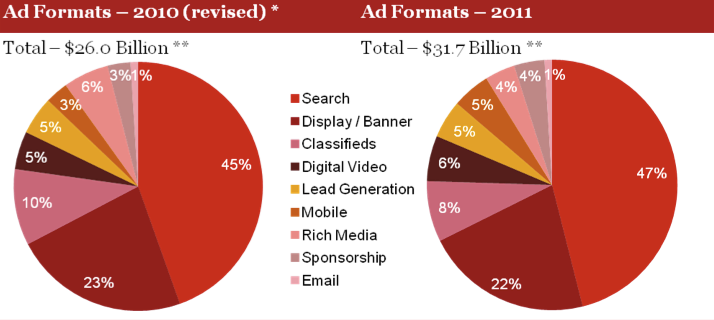
\includegraphics{chapter2.tex/Image0}
  }
\caption{Revenue According to Ad Format \citep[Image credit: ][]{IAB:sv1S8BTo}}
\end{figure}

\begin{sloppier}
Because advertisers are most concerned with efficiently reaching high value consumers (those most likely to buy), targeting is important across all forms of advertising. On the surface, targeting is about breaking the market down into groups, or segments, which share certain characteristics. Typical market segments includes geographic (e.g., region, climate, urban / surburban / rural), demographic (e.g., age, gender, ethnicity, education), contextual (e.g., web page content) and behavioral (e.g., browsing history, content accessed over time). Ideally, advertisers target an advertisement to users most likely to be influenced by it. To accomplish this, advertisers attempt to collect and correlate information about users in order to best segment them. 
\end{sloppier}


Intrinsically, targeting seems linked with profiling and the potential for the accumulation, aggregation, and storage of personal data. Advertising networks claim that such information is anonymous, while consumers and policy makers struggle with the question of whether advertising networks should be entitled to assemble profiles and whether that should entail gaining user permission first. In this balance of this section of Chapter 2, we will put aside privacy concerns and instead focus on:

\begin{enumerate}
\item What it means to track users and why this is important;
\item The nature and use of behavioral data in advertising; and,
\item New market opportunities and potential effects.
\end{enumerate}


\subsection{Tracking Users}
\label{trackingusers}

Defining ``tracking'' is a contentious exercise. The World Wide Web Consortium (W3C) Tracking Protection Working Group has been struggling with a definition for over a year (W3C, 2012). But, in its broadest sense, tracking is the collection, correlation, or transfer of data about Internet activities of a particular users, user agent, or device. Tracking may or may not be consensual and the users may or may not be aware of who is tracking, how tracking occurs, or what data is tracked. Tracking in the browser is most commonly associated by the use of HTTP cookies, but other means include IP address tracking, flash cookies (using the Adobe Flash plug-in), and web bugs or beacons (e.g., images retrieved from a third party website). Of potential future concern may be browser fingerprinting  \citep{Eckersley:2010uj},  though it does not seem that advertisers are using this technique now.

Publishers and advertisers alike track user data. Publishers, or first-party, tracking may include very fine-grained information about a user such email address, name, navigation behavior, etc. Personally identifiable information (PII) may be collected with user consent. And companies with both a brick-and-mortar and significant online presence likely combine information about what they know from shopping habits in the store with other data obtained online. More recently, even purely online businesses are able to tap offline data. For example, FaceBook has recently partnered with Datalogix to link online and offline consumer data  \citep{Reitman:2012wc}. 

First party tracking may also be combined with data collected and aggregated by third party trackers. Third party trackers do not communicate directly with a user but monitor a user's actions in other ways. Generally, third party trackers are explicitly given consent to track by a website publisher. But they may also acquire user data via data exchanges and from Internet Service Providers (ISPs; e.g., via deep packet inspection such as that described in  \citealp{Sesto:2008va})  or other vendor sources. It is also possible for trackers to acquire data by taking advantage of security vulnerabilities and via information leakage (as described in  \citealp{Krishnamurthy:2009vh},  for example).

\subsection{The Nature and Use of Behavioral Data in Advertising}
\label{thenatureanduseofbehavioraldatainadvertising}

In fact, how behavioral tracking is accomplished is anything but transparent. The image below in  \autoref{http}  depicts the many HTTP requests called from the New York Times (NYT) homepage in November of 2012. 


\begin{figure}
\centerline{
  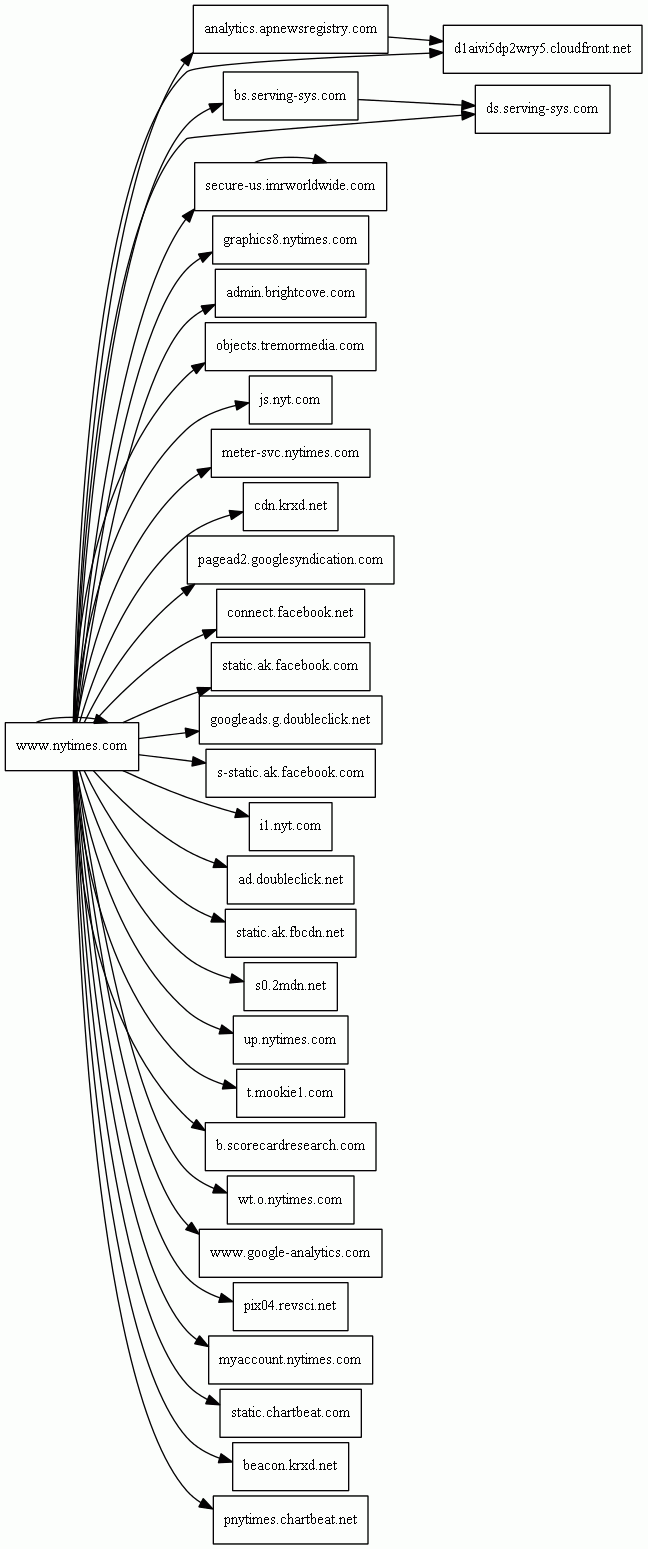
\includegraphics{chapter2.tex/Image1}
  }
\caption{HTTP Requests from the New York Times Homepage}
\label{http}
\end{figure}


A large number of the domains included are third party trackers engaged in analytic or personalization services and advertising. But what makes behavioral tracking feel so insidious is that user activity on one site \emph{can directly influence content displayed in completely un-related sites}. 

For example, on October 5, 2012, after visiting the NYT, Washington Post, and Mozilla home pages, I generated a search query for ``waterproof boots'' on Google search. On October 6, 2012, I refreshed the NYT homepage and was presented an ad for Marc Jacob waterproof boots prominently displayed in the top banner ad space in  \autoref{boots}  below. This may or may not be co-incidence. There is no way to know.


\begin{figure}
\centerline{
  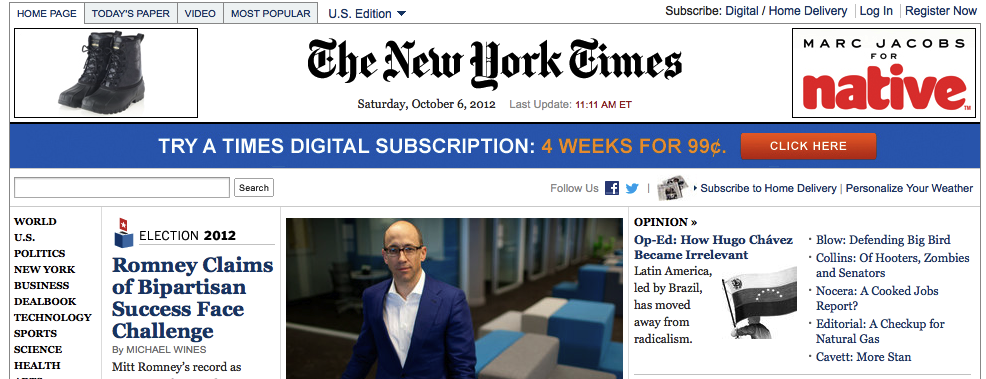
\includegraphics[scale=.75]{chapter2.tex/Image2}
  }
\caption{New York Times Homepage with Advertisement for Marc Jacob Boots}\label{boots}
\end{figure}


A graph diagram generated from the Firefox Collusion extension in  \autoref{collusion}  offers few clues about how my Google query might have caused this ad to be displayed on the NYT homepage. 


\begin{figure}
\centerline{
  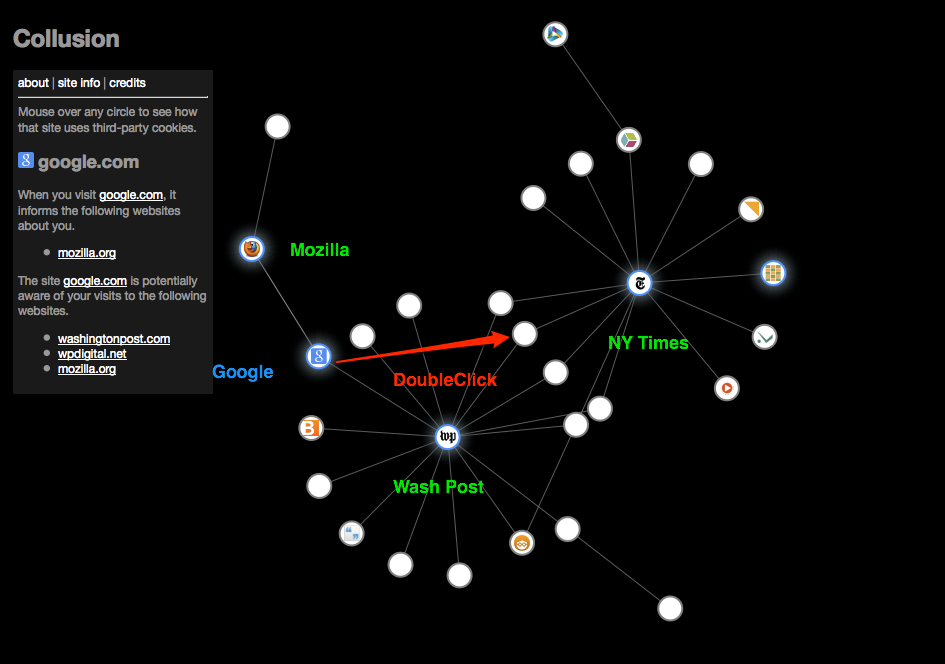
\includegraphics[scale=.75]{chapter2.tex/Image3}
  }
\caption{Firefox Collusion Diagram}
\label{collusion}
\end{figure}


Possibly, Google's advertising subsidiary DoubleClick may have been involved. When seen in the context of this collusion diagram, DoubleClick appears to know of visits to the Washington Post and NYT, but not what search query was made. Yet this is still possible. Business relationships outside of the communicative context also account for data transactions and exchanges.

Behavioral tracking concerns technologies and methods centered on capturing user data when users interact with web content. For example, information captured may include: user visits to a web site, specific page content, visit recency \slash  frequency of visits, links clicked, searches, form data, and other interactive content. This data, plus metadata such as IP address may be combined to create a `profile' linked to that user, browser user agent, or device. The goal of behavioral targeting is to show ads only to users of high value (those who are likely to buy the product) combined with a large number of opportunities to show such ads to that user.

An informal survey of agencies by the IAB suggests that behavioral advertising is widespread: up to 80\% or more of advertising campaigns conducted in 2009 involved some form of tracking  \citep{IAB:2010wz}.  But until recently, we've had little real insight into how businesses, to include advertisers, used behavioral tracking.

In Feb 2012, The New York Times published an article written by  \cite{Duhigg:2012ua}  telling the story of how Andrew Pole, a data scientist in Target's marketing analytics department, developed a model that could successfully predict whether a female customer was in the second trimester of pregnancy.

According to  \cite{Duhigg:2012ua},  there are periods in life when routines and buying patterns change. Advertisers are quick to target customers during major life changes such as the purchase of a house or vehicle, or birth of a child. Retailers are particularly interested in acquiring and retaining new customers during such life changes when habits are more malleable. In the case of a birth event, parents will buy all sorts of items such as maternity clothing and prenatal vitamins --- transitioning to baby care products soon after. Pole began analyzing consumer spending to identify 25 products, in aggregate, predictive of pregnancy and within a narrow window of time. As  \cite{Duhigg:2012ua}  notes, ``it's difficult to attribute how much behavior modeling contributed to Target's revenue, but between 2002 --- when Pole was hired --- and 2010, Target's revenues grew from \$44 billion to \$67 billion''  \citep{Duhigg:2012ua}.  Beyond anecdotal accounts such as pregnancy prediction by Target, there is relatively little information available about how businesses and advertisers profile users through online tracking. 

Not all businesses have such fine-grained information as customer data to enrich predictive models. While Target may have access to name, address, demographics, geography, contact history and many other pieces of information  \citep{HowTargetGetsthe:2010wu},  search engines typically have access to different sorts of data. In  \cite*{Yan:2009dk},  a team from China reportedly published the first academic, and empirical study, to address the question of the whether online behavioral targeting (OBT) can help in online advertising. In this paper, a basic OBT assumption was addressed. The basic assumption is this: ``users who have a similar search or browsing behavior will have similar interests and thus have higher probability to click the same ad than the users who have different online behaviors''  \citep{Yan:2009dk}.  

The team used seven days' ads click-through log data from a commercial search engine recording user search click behavior to include both web page clicks and ad clicks. They represented user behavior by page views and created a behavioral profile by considering all terms appearing in a user's query as previous behaviors. Both users and queries were represented as numerical vectors so that similarity between users could be easily calculated. Using simple clustering techniques, users were segmented according to behavior. Finally, user within-ad similarity was compared with user between-ads similarity. The result was that the within ads similarity, represented by user search behavior, was around ninety times larger than between ads similarity. Thus  \cite*{Yan:2009dk}  concluded that users with similar search behavior would indeed be distinguishable from other users and this could be used to predict the clickability of an ad.

 \cite*{Chen:2009jb}  described ``massive improvements'' in the ability to do offline training of OBT models. They noted, ``behavioral data is intrinsically in large scale (e.g., Yahoo! logged 9 terabytes of display ad data with about 500 billion entries on August, 2008)'' with a sparse click through rate (CTR) of about 0.05\%  \citep{Chen:2009jb}.  To build the entire 450 OBA category models from Yahoo! on fine-grained (ad clicks and search queries) at this scale would take about a week before the innovations they describe were implemented. By using a MapReduce learning algorithm, improved feature vector generation algorithm, better in-memory caching, and more efficient data structures and models they were able to reduce offline model building to about one day.

Scarcely a year later,  \cite*{PandeyΟ:2011ug}  demonstrated the ability to include even more behavioral context to achieve, what they describe, as better results on live data. They created a general purpose model which allowed for optimizing three strategies of behavioral targeting: property (document context), segment (user demographics), and behavior (user past behavior). Each strategy was estimated to successively encode deeper context, thereby potentially improving the richness of the model. User events were modeled as an event stream of three types of events: pages visited, search queries, and graphics ads. By modeling in this manner, the research team examined the relative performance of specific event types (using extracted features), within specific temporal windows with respect to a variety of advertising campaigns of various types and sizes.
In a live experiment spanning three months, they generated user models spanning eight weeks of user history. For each of four ad campaigns, old models (like those described in the previous two paper described above) and new models received at least 1M ad impressions on a monthly basis. The conversion rate for new models was calculated to be considerably higher than for the older models, ranging from 57\% to 264\% higher.

 \cite{PandeyΟ:2011ug}  note, the problem of predicting clicks and predicting conversion have been split along clear lines of information available to publishers and information available to advertisers. There has been growing pressure from within the ad industry to change this. Moving to payment by conversion is an attractive option for advertisers because: 1) it helps to prevent click fraud; 2) can be used to analyze the effectiveness of the advertisement (was there an actual sales conversion and not just a click); 3) can prevent the user from being inundated by too many of the same ad; and, 4) and is compatible with re-targeting across sites  \citep{PandeyΟ:2011ug}.  Accordingly, advertisers have been recently more willing to share individual responses to ads to publishers since it facilitates the use of conversion-optimized models.

\subsection{New Markets}
\label{newmarkets}

The market of online advertising today is, in fact, much more complex than simple supply (publisher) and demand (advertiser) economics. This model, known as direct buy, was dominant in the early days of online advertising  \citep{Mayer:2012wt}.  By the late 1990's advertising networks emerged allowing advertisers to place ads with many publishers --- and publishers to work with many advertisers --- through a common network. In such a model, it is easier for advertisers to target users along multiple dimensions (e.g., page context, demography, geography, behavior) for ad slots.

The advertising community as a whole sees targeting as an opportunity funnel (see  \autoref{facebook}).  Relating this back to psychology, advertisers are aware that to target effectively, then need to consider consumer:

\begin{enumerate}
\item Daily activities;
\item Online activities and habits; and
\item Research time, whether purchase is online or offline \citep{Anonymous:2010uw}.
\label{opportunity}
\end{enumerate}


There is a clear ``in market'' time of opportunity when users are researching purchase decisions. During this period of time, their behavior changes in predictable ways. For example, initially, the user may broadly review a general product space. Then move to a more comparative or winnowing down of choices. And finally, that consumer will look for a store and make a purchase.

Cookie re-targeting takes advantage of this purchase funnel. Recently, Facebook announced a new Facebook Exchange program, a real-time bidding ad system, where visitors with exchange party cookies can then be shown ads related to their web browsing when they return from those sites to Facebook  \citep{Constine:ut}.  The basic idea is to re-target customers that visited a commercial site but did not purchase at that visit. This effectively positions Facebook from working in the broad part of the funnel (demand generation) to the more narrow part of the funnel  \citep[demand fulfillment;][]{Constine:ut}. 


\begin{figure}
\centerline{
  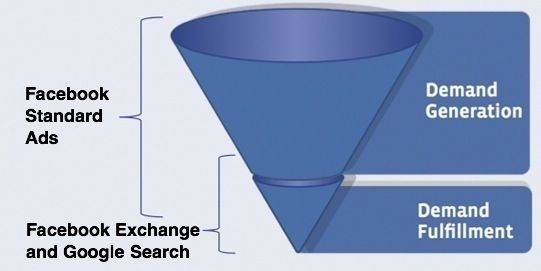
\includegraphics[scale=.75]{chapter2.tex/Image4}
  }
\caption{Facebook Re-targeting \citep[Image credit:][]{Constine:ut}}
\label{facebook}
\end{figure}


To do this, Facebook doesn't share biographical information with advertisers, but takes cookies and combine them with Facebook data  \citep{Constine:ut}. 
The emergence of an \emph{exchange market} --- where buyers and sellers converge --- is attributable to Google's DoubleClick Ad Exchange in 2009  \citep{Duggal:2012tq}.  The perceived value of an exchange over an advertising network is that the exchange operates on the behalf of any number of buyers, sellers, and middlemen alike.  \cite{Anonymous:2012uw}  estimates that real-time bidding exchanges now account for 40\% online data collection. This is up from 0\% three years ago.

Another sort of emergent market is a data market. \emph{Data management platforms} serve as ``a unified technology platform that intakes disparate first-, second-, and third-party data sets, provides normalization and segmentation on that data, and allows a user to push the resulting segmentation into live interactive channel environments''  \citep{OConnell:2011tq}.  Krux  \citeyearpar{Anonymous:2012uw}  found that more than 300 companies collected data on its users, up from 167 companies in 2010. 

Many data collectors also piggyback on each other. By piggy-backing, one tracker invites other trackers to the trough. Because of this, publishers and users may not be aware of how much data is tracked on a given site  \citep{Angwin:2012tg}. 

Not surprisingly, it is difficult to measure the effect of behavioral advertising. Referencing a study from  \cite{Kazienko:2007tb}, \cite{Farahat:2012ex}  observe that click-through-rates (CTR) have declined from 3\% to less than 1\% (since the 1990s). CTR have traditionally been a measure of ad performance, though ultimately, advertisers prefer a more concrete measure such as sales conversions. In the  \cite{Yan:2009dk}  experiment described earlier, ad CTR improvements through behavioral tracking were measured as high as 670\% on the basis of their simple user segmentation strategy from search queries and clicked pages.

However,  \cite{Farahat:2012ex}  question these ad CTR results stating that any study that naively looks at response lifts between targeted and un-targeted groups will greatly overestimate the effects of advertising since there is an inherent selection bias: the targeted users' behavior is likely to be highly correlated with the measured response (``click'').  \cite{Farahat:2012ex}  ask, how do you know that the targeted segment isn't also the most clicky? Since what advertisers care more about are sales conversions than clicks, this is an important question.

In a field experiment on the Yahoo! front page,  \cite{Farahat:2012ex}  try to weed out selection effects in terms of clickiness of the targeted population, brand interest, and category interest. They find strong evidence that user clickiness and brand interest are determinants of variation in CTR. This has bearing on the projected ROI of behavioral advertising for a given campaign. Furthermore, they question the ad CTR improvements of  \cite{Yan:2009dk},  suggesting that the targeted lift of brand-related searches may be over-estimated by almost 1000\%.

 \cite{Farahat:2012ex}  conclude that advertisers would benefit from comparing how targeted and non-targeted populations respond to advertising in any particular campaign in order to gauge the cost effectiveness of their targeting strategy. ``Given an industry average of a three times price premium for targeting, we might conclude targeting is more cost effective, but of course this depends greatly on the targeting product''  \citep{Farahat:2012ex}.  To date, relatively little is published about proprietary behavioral tracking model development nor the effectiveness of such models in actual ad campaigns. Nonetheless, the value of behavioral data is vigorously defended by marketers in public media as ``the fuel the drives the Internet''.\footnote{This is an oft repeated phrase in the media and not attributable to a particular person or source.}

What we really have little understanding is how to deal with the socio-technological effects of the connectedness of many different sorts and bits of data across vast networks of inter-connected participants. Currently, the heavy emphasis is on \emph{who} to target. But there is mounting research to suggest that \emph{when} (in the purchase funnel), \emph{where} (on what site and how the ad should be placed), \emph{what time of day}, \emph{at what geographic location}, \emph{how often}, and \emph{how much} to pay (via auction strategy) are also important to advertisers. Furthermore, with the market moving away from CTR (click through rate) and CTM (cost per mile \slash  ``impression'') towards a sales conversion rate (CVR), there will pressure for even greater information flow between producers and advertisers. Impediments to behavioral tracking become no longer technological, but sociological. And of course, these barriers will fall if both producers and advertisers believe they can profit.

In purely statistically-driven systems, the amount of data, not the algorithm, is king. However, there are many examples of where social network topology provides information that dramatically improves performance over pure volume. When Google created the PageRank algorithm it used page outbound links as implicitly encoded information about what page creators thought important. So what might the effect be when social networks such as Facebook harness vast networks of inter-connected consumers to the problem of behavioral advertising? How likely are we to behave like our friends? Or to what extent can they be used to influence us?\footnote{A NYT article (published Oct. 13, 2012) reports on how the current presidential political campaign is heavily leveraging social and behavioral information to both reach ``in market'' voters as well as pressure them to vote.  \url{http://www.nytimes.com/2012/10/14/us/politics/campaigns-mine-personal-lives-to-get-out-vote.html?pagewanted=1&hp&_r=0} } What if producers and advertisers find secure and effective means of sharing private information about users and their purchasing and other behavior? If the time has not yet come that transactional, behavioral, social, geographic location, and other offline third party data sources are not combined and used by business to more closely target individual consumers --- that time will come shortly.

\section{Privacy and Policy Issues}
\label{privacyandpolicyissues}

Every day, major newspapers across the globe report on some concern over digital data and privacy. Included in this global discussion are talk of law, policy, and technology --- to include threats to privacy as well as proposed solutions. According to  \cite*{Gomez:2009ue},  consumer reports and polls repeatedly show ``overwhelming concern by users about the collection of personal information and behavioral profiling''  \citep[p. 17]{Gomez:2009ue}.  While website publishers typically offer a privacy policy to inform consumers what sorts of data may be collected and how that data may be used or shared, there is nonetheless much confusion and debate regarding what data is considered private and how it is handled. Though how personal data is collected and stored by first-party websites is in question, this section focuses more on the problem of data collected and used by third party trackers as well as public attitude toward this collection. However, in current privacy debates, there has been intrinsically little difference in the stance and attitude between large publishers and advertisers.

\subsection{The Internet is Free}
\label{theinternetisfree}

For some years, the Internet has been a free and open place. Access to services and information has been largely free. While many were initially skeptical about online commerce, convenience and ease won us over. With the advent of mobile technology and GPS, our applications became time and location aware. We can scan barcodes in stores and have applications tell us whether cheaper products are found close by. We embrace the wonder of connecting our virtual lives with our physical lives. But we feel uneasy, as well. The idea of being personally \emph{surveilled} as we move about in the physical world is deeply unsettling --- whether at home or in public. But to be monitored in a web browser leaves open the possibility that strangers will learn, in an intimate sense, \emph{who we are}. They will do this by knowing what we read, what activities we pursue, where we live and travel, where we bank, where we work, what sorts of medical issues we research --- and, naturally, what we buy. This information can be aggregated and stored by strangers --- and then shared with other strangers: without consent, without review.

The delicate balance between public and private life may, in fact, be a relatively recent phenomenon.  \cite{Locke:2010wt}  examines closely the inherent tendencies of biological organisms to eavesdrop on others. Privacy is likened to a ``regulatory process that serves to selectively control access of external stimulation to one's self or the flow of information to others''  \citep[p. 53]{Klopfer:1977ch}.  One of the key functions of privacy is the withholding of information that might provide an opponent with a competitive advantage  \citep{Klopfer:1977ch}.  

In small, egalitarian societies, the ability to constantly monitor and eavesdrop ``rendered trust unnecessary''  \citep[p. 74]{Locke:2010wt}.  Everyone shares access to the same resources. According to Locke, the pervasiveness of eavesdropping serves as a form of social control with an inhibitory effect on behavior. In more complex societies, where walls and buildings function as a sort of social technology, it has become less possible to overhear others and the notion of privacy has became mired with secrecy. At the same time, since one does not know everyone in the community, eavesdropping has become a means for knowing and understanding the private lives of others. Ultimately, ``walls and population increases made it necessary to take in information about others when they were physically absent, relying on the representations --- the gossip --- of intermediaries''  \citep[p. 192]{Locke:2010wt}.  


\subsection{Privacy and Personally Identifiable Information (PII)}
\label{pii}


Dan Solove, a George Washington University Law professor and author of \emph{Understanding Privacy}  \citeyearpar{Solove:2008vz},  frames privacy in terms of legal history and case law. The Fourth Amendment provides for the fundamental right to a ``reasonable expectation of privacy'' to the United States Constitution  \citep[as cited in][p. 2]{Solove:2008vz}.  In Katz v. United States, 1967, the Fourth Amendment protection was extended to include Fourth Amendment protection to public places, such as private conversations in public phone booths  \citep[as cited in][p. 22]{Solove:2008vz}.  However, the Supreme Court observed, ``What a person knowingly exposes to the public, even in his own home or office, is not a subject of Fourth Amendment protection''  \citep[as cited in][p. 22]{Solove:2008vz}. 

In fact, it is the inherent difficulty in resolving what ``privacy'' is, that drove Solove to write his book. He notes ``there is no overarching conception of privacy --- it must be mapped like terrain, by painstakingly studying the landscape''  \citep[p. ix]{Solove:2008vz}.  This is particularly relevant when considering user browser-based interaction with websites over the Internet.

As  \cite{Solove:2008vz}  notes, there are literally hundreds of laws at state and federal levels to protect privacy:

\begin{quote}
Congress has passed several dozen statutes to protect the privacy of government records, student records, financial information, electronic communications, video rental data, and drivers' records, among other things. Furthermore, privacy is recognized as a fundamental human right. According to the United Nations Declaration of Human Rights of 1948, "No one shall be subjected to arbitrary interference with his privacy, family, home or correspondence, nor to attacks upon his honor and reputation." \citep[p. 3]{Solove:2008vz}.
\end{quote}

At particular risk or bits of information known as ``personally identifiable information'' (PIIs) typically associated with harms such as identify theft and mis-use. In May 2007, the Deputy Directory of the Office of Management and Budget (OMB) sent a memorandum on the subject of ``safeguarding against and responding to the breach of personally identifiable information'' noting,

\begin{quote}
The term "personally identifiable information" refers to information which can be used to distinguish or trace an individual's identity, such as their name, social security number, biometric records, etc. alone, or when combined with other personal or identifying information. \citep{OMB:2007vu}
\end{quote}

The purpose of this memorandum was to reinforce requirements of the Privacy Act of 1974 to both safeguard and establish rules of conduct for the handling of personally identifiable information. The particular challenge was in response to the ease to which technology has made it possible to personally identify particular individuals by combining small pieces of information. It is not that this is a new challenge: for example, brick-and-mortar businesses have long asked customers for a zip code when a customer pays with a credit card. These two pieces of information can be easily combined to find a home address. What's changed is that technology and the Internet has made it far easier to identify and, potentially harm, users at vast scale. And the idea of PII now seems to extend to seemingly innocuous bits information such as Internet browsing behavior. What was once viewed as categorically deterministic is now probabilistic in terms of re-identifiability and risk.

\subsection{Growing Public Awareness}
\label{growingpublicawareness}


\begin{quote}
\textbf{Steward Cheifert} (Interviewer): How concerned should I be as a user about what I put up on the Net?

\textbf{John Markoff} (West coast correspondent, New York Times): I think it depends on what you do. There's better security coming for economic business transactions, but I'd be careful about putting my password on the net, I'd pick a password that's a safe password, and I wouldn't put my credit card up until there is security software up that will protect my credit card. \citep{TheInternet:uu}
\end{quote}


In the early 1990's, the Internet exploded into public awareness. 1993 signaled the first graphical web browser and the world was mesmerized. There was a growing excitement for interaction on the World Wide Web, and public talk was dominated by the promise of possibility. The large concern was whether it was safe to shop online --- though the focus was on the encryption of credit card transactions, rather than the seemingly benign micro-exchanges of a user clicking through web pages. 

In November of 1999, DoubleClick, an advertising network of over 11,000 publishers, purchased Abacus Direct a company maintaining a database of detailed consumer profiles on approximately 90\% of American households  \citep{Anonymous:Hkl3lUXG}.  DoubleClick announced that it planned to merge ``anonymous'' online data (100 million user profiles) with Abacus profiles (including names, addresses, phone numbers, etc.). The media roiled and public sentiment was overwhelmingly negative. Ultimately, DoubleClick put these plans on hold: it's stock dropped dramatically after the merger was announced since neither the public nor Wall Street had reacted favorably to this plan  \citep{Anonymous:1999wh}.  It was about this time that the public became aware of how their behavior on the Internet might be used by commercial entities. A Federal Trade Commission (FTC) investigation in 2001 ended its investigation with no finding that DoubleClick had engaged in unfair or deceptive trade practices. It concluded:

\begin{quote}
Based on this investigation, it appears to staff that DoubleClick never used or disclosed consumers' PII (personal identifiable information) for purposes other than those disclosed in its privacy policy. Specifically, it appears that DoubleClick did not combine PII from Abacus Direct with clickstream collected on client Web sites. In addition, it appears that DoubleClick has not used sensitive data for any online preference marketing product, in contravention of its stated online policy \citep{Anonymous:Hkl3lUXG}.
\end{quote}

This case, and others like it, now had the public's eye. By the year 2000, 54\% of Americans used the Internet at home  \citep{Simms:2000vo}.  In a March 2000 poll, 82\% of web users polled indicated that they were uncomfortable if their browsing habits and shopping patterns were linked to their identities  \citep{Anonymous:te}.  74\% indicated that they were very uncomfortable if their information were sold to other organizations. Though only 40\% of users had heard of browser ``cookies'', many were aware that data was being collected silently and that data could be both sold and merged with identifiable information. Public negative sentiment toward tracking has changed little over the years. Over 70\% in 2012 say they find little value in online ads  \citep{Hoofnagle:2012uc}.  And Microsoft reports that 75\% of its US and European users would like to opt-out of online advertising  \citep{Hill:2012uh}. 

\subsection{Third-Party Data Collection}
\label{third-partydatacollection}

Browser tracking is not the only means by which websites identify and collection user information. But it's, perhaps, the sort of data collection people are intuitively least comfortable with. Third-party trackers are trackers on websites that collect information about users for a third party. They are not officially part of the website visited, but are generally associated with advertisers or web analytics. Typically, they take the form of cookies. Cookies can be set by embedded JavaScript and allow a site to essentially ``remember'' arbitrary bits of information from a previous session. Advertisers can utilize cookies in a cross-domain manner by creating a unique ID that is set by one website and then picked up by that same advertiser on another website. In this way, the advertiser knows that you've visited both sites. 

The problem with cookies is that it is a browser-mediated information exchange \emph{hidden from view}. Some cookies serve useful functions for sites with which we have trusted relations. But many are set and tracked by organizations that we may not recognize and for purposes that are unclear. Of great concern is that these entities may be buying, selling, and trading browser profiles which can be linked to personally identifiable information (PII).
 \cite{Narayanan:2011tv}  proposed a five-fold taxonomy in which browsing history might become pseudoanonymously\footnote{``Psuedoanonymous'' unique IDs may be used to identify a particular device or user agent. These may potentially be linked to other, personally identifying information later.} identifiable to a particular device or user.

\begin{enumerate}
\item \textbf{The third party is sometimes a first-party.} A third party tracker such as Facebook may be a first-party in other contexts. If you visit Facebook and login, it sets a cookie that can be used to track you as you browse the web. \cite*{Roesner:2012uj} describe the particular situation where sites have buttons such as Facebook, Twitter, or Google embedded on their web pages. These buttons are trackers and used to track you even if you never click on them. If you visit a website, and are also logged into Facebook in the same browser, Facebook will know that you've visited that site.
\item \textbf{A first party leaks data to third-parties.} \cite*{Krishnamurthy:2011uv} found that 56\% of 100 popular, non-social network sites leaked private information. This number grows to 75\% if a site userid is included as a PII.
\item \textbf{A first party sells the user's identity.} The previously mentioned case of Abacus and DoubleClick serves as a good example. Also, \cite{Narayanan:2011tv} notes that survey sites (e.g., "win a free iPod!") can also act as an identity provider to sites on which they have a third-party presence.
\item \textbf{Hacks and exploits.} A third-party might exploit a cross-site vulnerability on a first-party website to learn the user's identity \citep{Narayanan:2011tv}.
\item \textbf{Deanonymization (re-identification).} A third party could match browsing histories against datasets to re-identify particular persons, as \cite{Narayanan:2010kb} did with the Netflix Prize dataset. In this experiment, they demonstrated that it's possible to identify a particular subscriber with only a little bit of information.\footnote{In fact, this is only one example of many. Re-identification is another huge challenge for privacy law. For discussion in greater depth, see \citet{Ohm:2010vj}.}
\end{enumerate}

Though Netscape never intended cookies to be privacy-invasive, enterprise-minded businesses quickly realized that cookies could be used for identifying browsers. In fact, the ecology of tracker technology in the wild is surprising complex and, potentially, adaptable.

 \cite{Roesner:2012uj}  performed a study in which they observed tracker behavior from the point-of-view of the client browser. They classified this behavior into five behavioral patterns in which a given tracker site might exhibit variable behavior depending on contexts. They note complex behaviors such as that of an aggregate tracker referring data to other trackers. A few trackers stored data in multiple locations simultaneously (e.g., cookies, flash storage, HTML5 local storage) or exhibited spawning behavior when cookies were cleared. When they asked the question of how much data can any one tracker could collect, using 2006 AOL search query data, they found that, on average, DoubleClick could track a user across 39\% of pages visited, and a maximum of 66\% of pages visited.

Though cookies are the most prevalent trackers, ``web bugs'' serve a similar function. They are traditionally embedded as small (often 1 pixel) GIF or PNG images and can also be used in HTML mail, informing advertisers whether an email has been opened and when. In March 2010, Ghostery identified 117 unique web bugs on nearly 400,000 unique domains  \citep*{Gomez:2009ue}.  Though privacy policies may state that information will not be shared with third parties, many of these sites nonetheless allow third-party tracking through web bugs  \citep{Gomez:2009ue}. 

Given the complex behavior of trackers, coupled with complex business practices in which first-parties and third-parties may mingle or exchange data, it is not surprising that users may be confused about who has collected, stored, traded, or used their browsing profile.

\subsection{Cookies and Privacy Law}
\label{cookiesandprivacylaw}

Recent litigation over OBT invokes Wiretapping acts both federal and state. At the federal level, the Electronic Communications Privacy Act (``ECPA'') Wiretap Act, Stored Communications Act (``SCA''), and the Computer Fraud and Abuse Act (``CFAA'') are frequently invoked. 

The federal Wiretap Act (as amended by the ECPA) protects the privacy of wire, oral, and electronic communication. The latter is defined as ``any transfer of signs, signals, writing, images, sounds, data, or intelligence of any nature transmitted in whole or in part by a wire, radio, electromagnetic, photoelectronic or photooptical system''  (\citeauthor{Anonymous:ux}).  Under  \S  2511(3), ``a person or entity providing an electronic communication service to the public shall not intentionally divulge the contents of any communications{\ldots} while in transmission on that service to any person or entity other than an addressee or intended recipient{\ldots}'' 

The ECPA has been criticized lately by the media:

\begin{quote}
Many Internet companies and consumer advocates say the main law governing communication privacy --- enacted in 1986, before cellphone and e-mail use was widespread, and before social networking was even conceived --- is outdated, affording more protection to letters in a file cabinet than e-mail on a server." \citep{Helft:2011wx}
\end{quote}

Such criticism had been directed at Government data requests, yet numerous cases solely involving commercial entities  abound.\footnote{For example, "In re Doubleclick, Inc." and others referenced at \url{http://www.internetlibrary.com/topics/electronic_cpa.cfm}.}  Of issue for OBT is an exception known as the \emph{consent exception}: so long as one of the parties of electronic communication has given prior consent to the interception, and the interception was not intended for criminal or ``tortuous act'', then it is exempt from the Wiretap Act  \citep{Anonymous:2008vj}.  

One notable case which invoked ECPA, SCA, and CFAA was the case of ``In re Doubleclick, Inc.''. In 2000, a class action suit was brought against Doubleclick Inc., which used cookies for behavioral advertising. With respect to ECPA Wiretap law, Doubleclick successfully argued that its affiliated websites were ``users'' of the Internet and that communications accessed by Doubleclick's cookies were ``of or intended for'' these websites  \citep{Anonymous:Hkl3lUXG}.  The Stored Communications Act was found not to apply to Doubleclick, as well. The SCA was intended to address temporary and transactional records of internet service providers. Cookies stored on personal hard drives and were out of scope for the intent of SCA  \citep{Anonymous:Hkl3lUXG}.  Finally, with respect to the Computer Fraud and Abuse Act, the plaintiff failed to provide evidence that they had incurred harm.

As it stands today, federal laws do not address concerns raised by online behavioral tracking on the Internet. Furthermore, given the single-party consent exemption of Federal Wiretap law, communications between Internet users and websites is not private if the website owner has given its consent for monitoring.

\subsection{Policy Legislation - Do Not Track}
\label{policylegislation-donottrack}

Though the United States does not have specific federal law that applies to behavioral tracking, the Federal Trade Commission (FTC) can enforce the terms of privacy policies under Section 5 of the FTC Act prohibiting ``unfair or deceptive'' marketing practices  (\citeauthor{Anonymous:vq}).  This applies to FTC handling of behavioral tracking. In 2011, the FTC found three parties in violation for the FTC act relating to third-party tracking  \citep{Mayer:2012wt}.\footnote{A violation is determined if a company states in a website notice or privacy policy that it does not engage in a particular practice, when in fact it does.} 

In 2010, the Federal Trade Commission proposed ``do not track'' technology as ``likely a persistent setting on consumers' browsers --- so consumers can choose whether to allow the collection of data regarding their online searching and browsing activities''  \citep{Anonymous:2010ti}.  This represents a form of self-regulation insofar that trackers are expected to respond appropriately to browser requests not to track. In its March 2012 report  \cite{Staff:2012th},  the FTC outlined a broader privacy framework to address a myriad of concerns surrounding data brokering, mobile, internet service providers, and enforceable self-regulatory codes. The scope of this framework applies to:

\begin{quote}
[...] all commercial entities that collect or use consumer data that can be reasonably linked to a specific consumer, computer, or other device, unless the entity collects only non-sensitive data from fewer than 5,000 consumers per year and does not share the data with third parties. \citep{Staff:2012th}
\end{quote}

The FTC notes that this framework applies to offline as well as online data and applies to data that is reasonably linkable to a specific consumer, computer, or device.

As proposed by FTC  \citep{Staff:2012th},  Do Not Track should include five key principles:

\begin{enumerate}
\item It should be implemented universally to cover all parties that would track consumers. 
\item The choice mechanism should be easy to find, easy to understand, and easy to use. 
\item Any choices offered should be persistent and should not be overridden if, for example, consumers clear their cookies or update their browsers.
\item It should be comprehensive, effective, and enforceable: it should opt consumers out of behavioral tracking through any means and not permit technical loopholes.
\item It should go beyond simply opting consumers out of receiving targeted advertisements; it should opt them out of collection of behavioral data for all purposes other than those that would be consistent with the context of the interaction (e.g., preventing click-fraud or collecting de-identified data for analytics purposes; \citealp{Staff:2012th}).
\end{enumerate}

Since the FTC released its preliminary findings, the W3C Internet standards body convened a working group toward the adoption of an industry-wide Do Not Track standard. This group includes representatives from the advertising industry, online businesses, academia, privacy advocates --- both nationally and internationally. The challenge for this group is to devise a standard that meets FTC guidelines, while satisfying a diverse array of agendas.

\subsection{Building Privacy Policies into Browser Protocols}
\label{buildingprivacypoliciesintobrowserprotocols}

In the late 1990s, there were a couple of attempts to address the problem of privacy invasion introduced by third-party cookies via technical means. Introduced in 1997, RFC 2109 was a proposal aimed at putting strict controls on cookie usage. Commercial entities participating in standards discussion objected to portions of this proposal and it was, ultimately, not supported by browser developers. ``Where the browser manufacturers had been asked to redesign their software to reject cookies automatically, Netscape and Microsoft Internet Explorer instead included options for users to reject cookies if they so chose''  \citep{Eichelberger:um}.  As cookie inventor Lou Montulli stated, ``browser default would still be set to accept cookies, since it was felt by the designers that if we were to unilaterally disable this feature, existing content on the Web would no longer work''  \citep{Bruner:1997ti}. 

From 1998 - 2003, the W3C organized a standards committee to propose a Platform for Privacy Preferences (P3P) standard  \citep{Schwartz:2009tc}.  The standard aimed to create a machine-readable policy that captured the complexity of human-readable privacy policies and boiled them down to a multiple-choice set of options. What resulted from long and heated discussion was highly controversial and touted as overly complex --- and unlikely to be adopted as a self-regulatory option with no degree of enforcement.

About the same time, advertisers began to take a more active role in self-regulation. The National Advertising Initiative (NAI) set up a website to allow users to download opt-out cookies for participating networks. Their principles have been to notify users and allow them a choice. Opt-out does not mean that you will not be tracked or that ads will not be served. It means that ads will not be tailored to your browsing behavior. Opt-out choices are stored in browser cookies, so they recommend to visit their opt-out page periodically for updates. 

Other advertising networks and companies have since also offered similar opt-out cookie  services.\footnote{For example, see \url{http://www.worldprivacyforum.org/cookieoptout.html}.}  Large advertising industry groups formed a new parallel self-regulatory program for behavioral advertising, the Digital Advertising Alliance (DAA). The DAA and the Interactive Advertising Bureau (IAB), a self-regulatory for advertising networks, advocate the use of an advertising option icon to be displayed on web pages with tracking scripts. A user who clicks on the icon sees a disclosure statement and can click through to an opt-out page. However, according to a 2011 study at the Center for Internet and Society at Stanford University, only 11.3\% of members to date offer cookie-based opt-out.  \citep{J:2011wm}. 

In 2007, the Center for Democracy and Technology (CDT) sent a note to the Federal Trade Commission (FTC) requesting that ``the online tracking and targeting of consumers --- both in its current form and as it may develop in the future --- needs to be limited so that consumers can exercise meaningful, granular preferences based on timely and contextual disclosures that are understandable on whichever devices consumers choose to use''  \citep{CenterforDemocracy:uc}.  They called for a national Do Not Track list similar to the national Do Not Call list. Their proposal called for a machine readable list of the domain names which used cookies and other means to track users. Browsers and third party software could then use this list in order to limit tracking  \citep{CenterforDemocracy:uc}. 

Thus, the W3C chartered the Tracking Protection Working Group (TPWG) ``to improve user privacy and user control by defining mechanisms for expressing user preferences around Web tracking and for blocking or allowing Web tracking elements''  \citep{Anonymous:vz}. 

In effect, discussion in this group mirrors, and perhaps fuels, public debate in media and society.\footnote{The public-tracking list is archived at:  \url{http://lists.w3.org/Archives/Public/public-tracking/}. } Chairs for the group serve to organize and moderate debate. As questions become more defined, formal ``issues'' are raised and ``actions'' assigned to particular members. For example, ISSUE--5, ``What is the definition of tracking?'' was opened on September 21, 2011. As of October 2013, there are 446 emails pertaining to this issue alone, and it is still open more than two years later. 

Because each member has his or her own platform or stance on any particular matter, debate sometimes bleeds into other venues. For example, as of this writing, the current DNT draft standard says the following (regarding determining a person's DNT preference): ``A user agent must have a default tracking preference of `unset' (not enabled) unless specific tracking preference is implied by the decision to use that agent''  \citep{Anonymous:uk}.  When TPWG member Roy T. Fielding, who works for Adobe but who also contributes to the open source Apache webserver codebase, committed a patch to this codebase which disabled DNT if the browser requesting data was Internet Explorer 10 (which at the time set DNT to 1 by default), he caused a ripple tide of effects. His patch, labeled ``Apache does not tolerate deliberate abuse of open standards''  \citep{Fielding:2012wh},  clearly reflects his own position on the implementation of DNT. This hit C\slash NET news and Twitter almost simultaneously. On Twitter, Jonathan Mayer  \citep{J:2012uz},  fellow TPWG member responded with  \autoref{tweet1}. 

\begin{figure}
\centerline{

\includegraphics{chapter2.tex/Image5}
}
\caption{{Tweet, 7 September 2012}}
\label{tweet1}
\end{figure}


About the same time, C\slash NET reported the event, noting Roy T. Fielding's position as an author of the DNT standard and principal scientist at Adobe Systems  \citep{Shankland:tz}.  Of course, there was an immediate back-lash on the public-tracking list between Mayer and Fielding, in which Mayer  \citep{J:2012vq}  partially retracted his comment on Twitter  \autoref{tweet2}. 


\begin{figure}
\centerline{
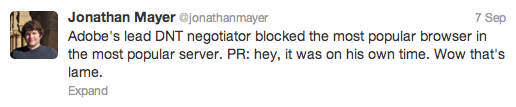
\includegraphics{chapter2.tex/Image6}
}
\caption{{Tweet, 7 September 2012}}
\label{tweet2}
\end{figure}


From Fielding on the public-tracking list:

\begin{quotation}
Our charter forbids us from specifying UI requirements. That does not mean any of the following excerpts are ambiguous:     

A user is an individual human. When user-agent software accesses online resources, whether or not the user understands or has specific knowledge of a particular request, that request is made "by" the user.

The goal of this protocol is to allow a user to express their personal preference regarding tracking to each server and web application that they communicate with via HTTP ...    

Key to that notion of expression is that it MUST reflect the user's preference, not the choice of some vendor, institution, or network-imposed mechanism outside the user's control. The basic principle is that a tracking preference expression is only transmitted when it reflects a deliberate choice by the user. In the absence of user choice, there is no tracking preference expressed. \citep{Fielding:2012vf}
\end{quotation}

On the basis of this personal conviction, Fielding argued that if DNT was switched on by default, it should be ignored, regardless of other considerations. Since Microsoft had announced that it would turn on DNT by default, Fielding retaliated using the technological means at hand --- direct modification of code. Naturally, this led to heated debate within the Apache http server developer community. As of this writing, there were 364 comments on this commit. Fielding's changes are reflected in the current configuration of the main branch of code, but are commented out.

Lorrie Craner, one of the original developers of P3P is skeptical that DNT will succeed. To her it seems a simpler, but not better, replay of the P3P proposal  \citep{Staff:2012th, Fulton:2012ti}. 

\begin{quote}
As we walk about in the physical world, we raise and lower our voice and we raise and lower our window shades and we turn our faces, and we are all constantly adjusting to regulate our exposure and our privacy, Dr. Cranor tells RWW. "And it comes naturally; we don't spend a lot of time thinking about it. We just sort of naturally do it. But when we go online, it's no longer natural, because we don't have these readily apparent, physical things where you can just easily close that shade, and it's obvious what you're doing. So we have to rely on software tools to help us with this privacy regulation process. \citep{Fulton:2012ti}
\end{quote}


\subsection{Choice and Self-Regulation}
\label{choiceandself-regulation}

While policy debate rages, the advertising industry continues to advocate self-regulation. Central to self-regulation is the notion of choice. The DAA and NAI naturally view behavioral advertising in a very positive sense such that better targeted ads are preferable to ads that do not match a consumer's interests. But if a user does not wish to participate, then they should have the choice to opt-out. However, privacy advocates cite two large concerns with respect to industry self-regulation.

The first argument against the effectiveness of self-regulation is non-compliance. A Carnegie Mellon University (CMU) report by  \cite*{Komanduri:2012wo}  finds that, despite attempts at self-regulation by bodies such as the DAA and NAI, there are still many examples of non-compliance. Stanford University website  \url{http://donottrack.us}  believes that further steps are required: namely, regulation enforcing compliance with user choice. 

A second, perhaps more compelling argument is that the advertising industry relies on technologies that seem to ensure that users remain unaware of them. When consumers attempt to block tracking, other more resistant methods are developed which circumvent these defenses. While DNT would make it very easy for users to decide not to be tracked, market choice seems to make it easier for them to be tracked. As  \cite*{Hoofnagle:2012ve}  note, ``those who argue that consumers can negotiate the nuances of privacy and tracking online assume that the online world is similar to the offline world.'' In the offline world the consumer can leave without leaving behind a data trail. But in the online world, invisible attributes leave marks that are easy to follow. They further note that surveys of top websites in 2009 and 2011, revealed new tracking mechanisms resistant to the strongest of privacy settings. Or, perhaps, advertisers simply know that once online shopping is habit, consumers will adapt.

\subsection{Opt-In Versus Opt-Out}
\label{opt-inversusopt-out}

On the 26th of May 2012 in the U.K., a new European Cookie Law, E-Privacy Directive 2009\slash 136\slash EC, came into effect.\footnote{There is a high-level summation here:  \url{http://gigaom.com/europe/cookie-law-explainer/}. } This law requires the consent of users before cookies are set (see  \autoref{cookie-notification}).  In effect, this is an unequivocal ``opt-in'' system of notification and consent (with the exception of cookies ``strictly necessary'' for the operation of a website  \citep{Anonymous:2009uu}.  


\begin{figure}
\centerline{
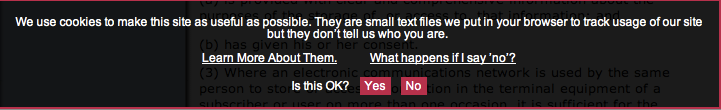
\includegraphics[scale=0.70]{chapter2.tex/Image7}
}
\caption{Example cookie opt-in notification from: \url{http://www.jonwallacedesign.com/privacypolicy.html}}
\label{cookie-notification}
\end{figure}


Unlike current trends in US policy and law, this puts the burden of consent on the website publisher --- not the user. Though this issue permeates the entire European Union (EU), discussion of the UK ``Cookie Law'' requirement for consent has finally reached US audiences on the Internet. 

Perhaps, this EU Directive gives a sense of what may be required if US lawmakers decide to place the burden of consent on website publishers and not users. Such a shift would also acknowledge that Internet transactions between users and websites are currently not ``private'' as Federal Wiretap law has held. The EU Directive seems more in line with user expectations, but given current criticism on the difficulty with compliance, falls short with respect to implementation. The hope is that the W3C Tracking Protection Working Group (TPWG) will provide strong enough guidance to satisfy this Directive. However, US members (and especially those representing business interests) may decide to act in an insular fashion and have, thus far, shown little motivation to join a more global debate  \citep{WCpublictracking:mGxHNO_D}.  

\section{User Confusion}
\label{userconfusion}

There has long been an asymmetry in communication between web publishers and users. Interactive page elements such as ``contact us'' via web forms, instant chat, web forums, and email have enabled users to connect directly to persons behind the scenes. More recently, publishers utilize personal messaging through other channels such as Twitter, Facebook, or SMS for allowing users to offer direct and personal feedback. These are direct and intentional communications between parties. But the act of visiting a webpage in itself also has communicative value. 

In this section, I highlight user confusion regarding indirect communications where advertisers and other commercial actors silently monitor web interaction via the use of cookies. Not only is the phenomenon of behavioral tracking difficult to understand and see, but user defenses against ubiquitous monitoring are confusing, as well. Of particular interest are user opt-out mechanisms provided for by emerging DNT standards and also the advertising industry efforts toward self-regulation of online behavioral advertising. The vehicle for this is ``consumer choice'' and the Advertising Option Icon (viz. AdChoices icon; see  \url{http://www.aboutads.info} for general information).  

\subsection{Confusion About Third Party Tracking}
\label{confusionaboutthirdpartytracking}

In a 2009 study of Internet user understanding of behavioral advertising,  \cite{McDonald:2009vz}  found that only 51\% believed that the ability of an ad company to determine which ads to show them based on the history of prior websites they visited was something that ``happens a lot right now'' \citep{McDonald:2009vz}.  46\% of the same study participants found the idea of behavioral advertising ``creepy'', and another 40\% agreed or strongly agreed they would be more careful online if they knew advertisers were collecting data.

In the virtual online world where billions of people have access to the web through the view of what may often be a personal device, it's not surprising that the experience feels, to some degree, private. As privacy advocate Christopher Soghoian remarks,

\begin{quote}
Consumers treat the search engine box like their psychiatrist, their rabbi, their priest, their doctor. People type the most intimate things into search engines and other websites primarily because they think they're anonymous. They type in things on WebMD that sometimes they wouldn't even ask their own doctors... And in fact, we are not anonymous, these sites are tracking us." \citep[as cited in][]{Kessler:2010vq}
\end{quote}


The UC Berkeley School of Information KnowPrivacy Project  \citep{Gomez:2009ue}  looked specifically at user concerns and knowledge. They examined 50 of the most visited websites and their privacy policies. They also considered specific practices such as third-party tracking and sharing with affiliates. Not surprisingly, they found that most users are concerned about data collection on themselves and their control over that collection and use of information. Furthermore, they found overwhelming evidence (from prior surveys) that users lack knowledge and understanding about data collection practices and policies.

Once source of obvious confusion has to do with terminology. What is tracking? Does that include collection? Most users think not  \citep{McDonald:2011vx, McDonald:2011uv}.  What is the difference between ``third party'' and ``affiliate''? Privacy law treats these categories differently: third-party information sharing is subject to more restriction. According to  \cite{Gomez:2009ue},  websites make distinctions between sharing with affiliates and third parties. 29 of 50 companies examined state that they do not share data with unrelated third parties, 45 state that they share data with affiliates, and 36 state that they allow third-party tracking. This last category falls outside of privacy policy coverage. As  \cite{Gomez:2009ue}  note, it's very unclear what it means to not share data with unrelated third parties yet permit third party tracking.

Despite assurances that affiliates and third parties are treated differently, website providers often leak personal information to the less trusted, embedded third party trackers such as username, login time, and other information. Just as troubling is that users have no practical way of knowing who affiliates are and what sorts of information are passed to them. In the Know Privacy Report  \citeyearpar{Gomez:2009ue},  many of the websites examined are owned by companies with hundreds of subsidiaries: NewsCorp has over 1500 subsidiaries while Bank of America has over  2300.\footnote{These numbers reportedly do not include subsidiaries of subsidiaries.}  The pervasive presence of third party trackers on the Internet means companies have ample opportunity to construct long term profiles of things we do online.

Privacy policies often go unread, or may be difficult to understand  \citep{Milne:2004dy, Sherman:2008uz}.   \cite{Fernback:2007bq}  conducted an in-depth discourse analysis of privacy statements of three large companies. They also noted discrepancies regarding the use of the term ``third-party''. From their study of the Real Network privacy policy: ``We will never sell, rent or disclose to third parties our customers' personally identifiable information {\ldots} gathered on a RealNetworks Website unless we are required to do so by law or receive your advance informed consent''  \citep{Fernback:2007bq}.  Yet, in what appears a blatant contradiction, later in the same privacy policy:

\begin{quote}
Your personally identifiable information may be transferred in connection with a sale, merger, transfer, exchange or other disposition (whether of assets, stock or otherwise) of all or a portion of a business of RealNetworks, Inc. and/or its subsidiaries. \citep{Fernback:2007bq}
\end{quote}

In general,  \cite{Fernback:2007bq}  note that privacy policies are seen to protect the company and typically avoid mention of specifics such as precisely what information might be collected and for what purpose. Given that the FTC has a history of prosecuting companies that violate their terms of  agreement,\footnote{See \url{http://www.ftc.gov/os/caselist/index.shtm} for example. Google and Facebook have both earned penalties.}  this is not terribly surprising. 

 \cite*{McDonald:2009vz},  examined the readability of online privacy statements. They examined standardized text formats and compared these to free text policies. They found that experiment participants could more readily read and comprehend standardized formats, but at the expense of accuracy. And users, in general, did not like either standardized or free text formats. But when it comes to purchasing privacy-sensitive items,  \cite*{Egelman:2009ut}  found that users actually paid attention to graphical privacy indicators.

\subsection{Confusion about Defenses}
\label{confusionaboutdefenses}

When it comes to defending against third party tracking and privacy, users have a number of choices.  \cite{Roesner:2012uj}  identified the following options:

\begin{itemize}
\item \textbf{Pop-up blockers:} Pop-up blockers can stop trackers from forced pop-ups, but there are similar methods such as site re-directs that may not be stopped;
\item \textbf{Browser third-party cookie blocking:} Many third party cookies can be blocked if users select third-party cookie blocking in their browers. However, this will not stop the sort of tracking when a Facebook tracker is accepted as a first-party tracker and its role changes later to a third-party tracker; 
\item \textbf{Private browsing:} Private browsing mode was designed to protect users from having their browse state examined by physical access. But it does not keep browsing state from being examined online;
\item \textbf{Opt-out cookies (and AdChoice icon):} The Digital Advertising Alliance (DAA) is an industry funded policy group that hosts an opt-out web page. From this page, users can click a button to set opt-out cookies;\footnote{There are other similar sites that offer opt-out cookies. For example, Evidon Global, and others have web pages with such links.}
\item \textbf{Clearing browser state:} Clearing cookies when closing the browser is a simple means to reduce the effects of tracking. However, this may also remove opt-out cookies and is also not effective against re-identification by trackers such as the Facebook like icon when logged in;
\item \textbf{Do not track (DNT):} The proposed FTC "Do Not Track" DNT policy is designed to give users a way to opt out of web tracking. This is accomplished via an http request header with a DNT=1 header to inform the remote server that the client wishes to opt out. DNT is not mandatory and requires no compliance. The DAA has committed only to stop content personalization, if it receives a DNT signal. (\url{http://www.aboutads.info/choices/}); and,
\item \textbf{Blocking plug-ins:}  There are a number of browser plug-in which are designed to block trackers.
\end{itemize}

Lorri Craner directs the CyLab Usability Privacy and Security (CUPS) Laboratory at Carnegie Mellon University. She and her students have conducted a series of studies centered on user understanding of online behavioral advertising and usability of blocking tools  \citep{McDonald:2010vv,Ur:2012ws,Leon:2012vu,Cranor:2012ui}. \cite{Leon:2012vu}  studied the usability of Ghostery, Adblock Plus, and the Internet Explorer Tracking Protection List blocking tools. They found that self-help blocker tools have significant issues in terms of user understanding:

\begin{sloppier}
\begin{itemize}
\item Users don't recognize the names of the majority of companies that they can opt-out;
\item Some of the tools use terms that were meaningless to participants: for example, "web tracker, web bug, flash cookie, silverlight cookie, tracking cookie, script, iframe, and targeted ad network.";
\item Participants testing opt-out tools did not understand what the tools would opt them out of, mistakenly believing that they were protected against tracking;
\item Opt-out tool users thought deleting cookies would protect their privacy even more, not realizing that deleting their cookies would also delete their opt-out cookies and undo their opt-out;
\item Users were left unaware whether or not most tools were working, and oblivious to what was happening behind the scenes;
\item None of the opt-out tools tested notify users while they are browsing that their preferences are being respected; and,
\item Participants who tested the browser cookie settings also had no mechanism for understanding what exactly was happening behind the scenes unless websites didn't work \citep{Leon:2012vu}.
\end{itemize}
\end{sloppier}

In a related study conducted by  \cite*{Leon:2012dk},  45\% of participants who saw ``AdChoices'' believed that it was intended to sell advertising space, while only 27\% believed that it was intended to stop tailored ads.
A significant part of the problem is that 1) users don't really understand the mechanisms behind tracking and so misunderstand the nature of the problem; and 2) users don't have a clear idea of what options are available to help alleviate the problem  \citep{McDonald:2010vv, Ur:2012ws}.  Moreover, users have no practical way of knowing how effective blocking is when it works.  \cite{Mayer:2012wt}  examined the effectiveness of 11 blocking tools and found significant variability in performance. Most of these self-help tools work about the same way. They consist of a black list that is modifiable by the user. The lists vary widely and account for much difference seen in performance. Since it's not obvious that these tools essentially work in the same way, users may be tempted to install more than one. However, doing so may be risky:  \cite{Mayer:2012wt}  report that TRUSTe's tool actually over-rode blocking lists by other tools allowing tracking by several large third party trackers.

\subsection{Are Privacy Concerns Affecting User Behavior?}
\label{areprivacyconcernsaffectinguserbehavior}

When questioned in polls and studies, users overwhelmingly share a negative attitude toward online tracking. In a 2010 CUPS study:

\begin{quote}
64\% found the idea invasive, and we see signs of a possible chilling effect with 40\% self-reporting they would change their online behavior if advertisers were collecting data. We found a gap between people's willingness to pay to protect their privacy and their willingness to accept discounts in exchange for private information. 69\% believe privacy is a right and 61\% think it is extortion to pay to keep their data private. Only 11\% say they would pay to avoid ads. We found participants are comfortable with the idea that advertising supports free online content, but they do not believe their data are part of that exchange. \citep{McDonald:2010wt}
\end{quote}

Though, a large proportion of users claim that they would change their online behavior if they believed advertisers were collecting data, there appears to be no general usage statistics to indicate that so large a population employs existing opt-out technology beyond what the browser may natively provide. In 2011,  \cite{Fowler:vx}  reported that only 5.6 of Firefox desktop users had turned on DNT. In terms of more aggressive blocking, when I started this dissertation in late 2012, 14 million Firefox users had installed the most popular blocker extension (Ad Blocker). But this was only approximately 3\% of the 450 million Firefox users which represented only 20--24\% of desktop browsers in use  \citep{Anonymous:KXG0mTUq, Anonymous:K3r7zLAx}.  However, trends do indicate that blocking trackers is growing in popularity  \citep{Acohido:2011ta}.  In late 2013, DNT adoption is approximately 17\% \citep{Fowler:dnt}.  And the new default setting for Firefox (as of Feb 2013) is not to allow all third party domains, but to allow cookies only from visited domains  \citep{Fowler:2013}. 

In some contexts, users may be willing to make very clear choices when confronted with a privacy trade-off.  \cite{Egelman:2009ut}  found that laboratory study participants of an online shopping task were willing to pay more for sensitive purchases when confronted with a choice between a site with less privacy but cheaper prices, and a site with more privacy but more expensive prices.  \cite{Hoofnagle:vy}  likewise found that more than half of online poll participants reported changing their minds about the purchase of a product online because of privacy concerns.

As users awareness grows, advertisers find new strategies to evade blocking  \citep{Soltani:2009vg, Leon:2012vu, Hoofnagle:2012uc}.  What users want is not in accordance with what publishers and advertisers are currently willing to do. In a survey from  \cite{McDonald:2011uv},  72\% expected that regulatory ``do not track'' efforts limit data collection, while 34\% of respondents expected that ``do not track'' would prevent data from being collected by websites and advertisers. Since industry proponents currently interpret ``do not track'' as not affecting data collection but simply use of data for presenting advertisements, there exists an impasse between consumer advocates and industry proponents in policy-oriented regulatory efforts by the W3C. 

Central to this debate is the notion of ``consumer notice and choice''. Advertising self-regulation is firmly based on this notion. As we will see in chapters to come, there are strong reasons why this is so.

\section{The Future of Interactive Advertising}
\label{thefutureofinteractiveadvertising}

Though the goal of advertising is ultimately to sell products, advertisers also have other goals such as gaining wider audiences and positive brand engagement. Interactive advertising plays a role in the space by providing consumers opportunities to interact with advertisements directly.

I live in the country. Recently, I was finally able to have high-speed Internet installed at my house. For the first time, I could stream broadcast content over my AppleTV. While I was poking around, I found I could access a PBS channel for free. In order to activate it, I was shown a code and asked to visit the PBS website to register. After registering, content was made available over my AppleTV. Now PBS knows who I am, what I watch, and when I watch it. Though, I am not engaging with ads over PBS yet, Apple has transformed the broadcast experience by opening a window between PBS and me, whereby we can affect each other's actions.

In the past year, we've seen other, more unusual, examples of interactive advertising. Lexus has created an ad which ``comes to life'' when an iPad is placed behind the printed magazine  ad.\footnote{\url{http://www.lexus.com/stunning}} 

\begin{figure}
\begin{center}
 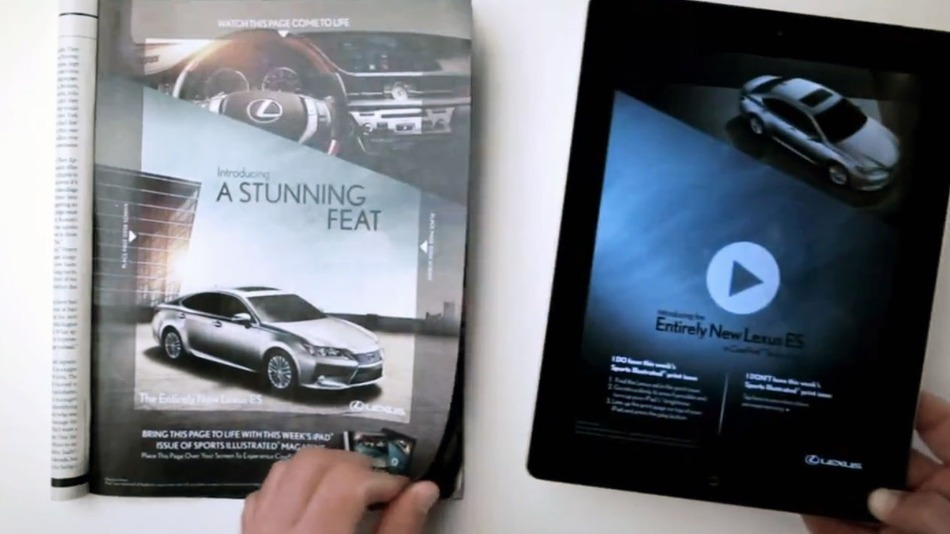
\includegraphics[scale=.50]{chapter2.tex/lexus}
\caption{Interactive Print Advertisement}
\end{center}
\end{figure}

Car manufacturers had already engaged a potential audience by creating game-like experiences where consumers could design their own vehicle and examine it in 3D. Cross-media experiences such as this, transform print into something new.

On October 5, 2012, \emph{Entertainment Weekly} placed a smartphone inside its print magazine. The phone contained a digital ad running video and live tweets  \citep{ulanoff:2013ma}. 

\begin{figure}
\begin{center}
 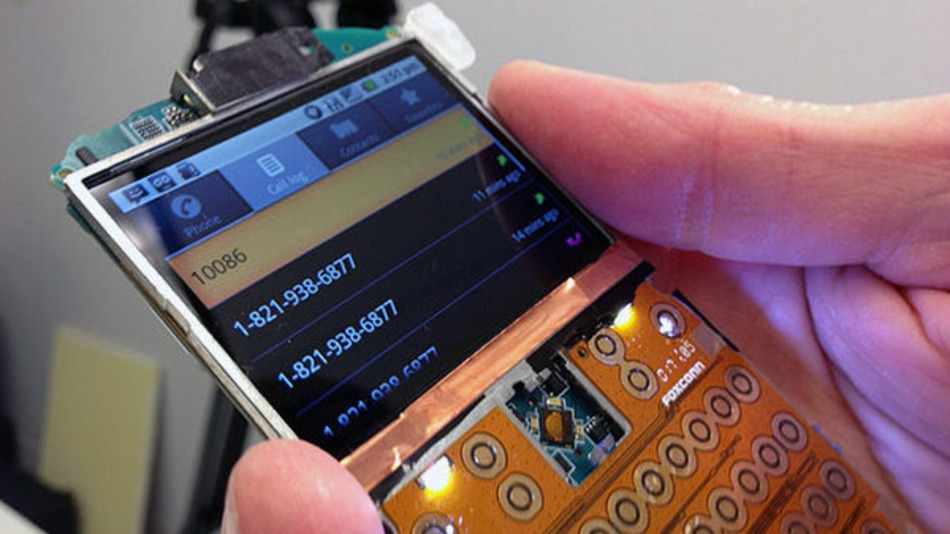
\includegraphics[scale=.50]{chapter2.tex/smartphone}
\caption{Print-Embedded Smartphone}
\end{center}
\end{figure}

It has become easier to imagine a world where print seems fluid and magic --- as envisioned by J.K. Rowling portrays the Daily Prophet in the world of Harry Potter.

Not surprisingly, there is a strong interest by advertisers to engage over mobile platforms. Utilizing location-based coupons, the iButterfly app engages customers by gamifying  coupons.\footnote{\url{http://www.cherrypicks.com/products/ibutterfly}}  Users flick their phone to hunt virtual 3D butterflies.

While interactive advertising may appear tangential to behavioral advertising, there is a common theme underlying both: \emph{interactivity}. Behavioral advertising relies on the ability to observe users engaging in everyday activities while interactive ads provide a means for advertisers to invite consumers to engaged with brands and products.

Why should this parallel concern us? It does not seem far-fetched to imagine the content of interactive ads become more tailored to the interests and expectations of individuals. Advertisers already argue that OBA benefits the consumer by delivering a more tailored (and presumably less annoying) experience. The argument posed by advertisers is fairly simple: wouldn't you rather see advertisements about products that interest you rather than advertisements about things that do not?

Suppose that advertisers collect images of your friends and family and create facsimiles which appear in  advertisements.\footnote{FaceBook may already use your posts and personal data for advertising \citep{goel:2013nyt}. Google also includes Google user names, faces, and content in ads \citep{kelly:2013cnn}.}  In June 2013, Alessandro Acquisti spoke of the following research in progress.

\begin{quote}
Imagine that an organization has access to your list of Facebook friends, and through some kind of algorithm they can detect the two friends that you like the most. And then they create, in real time, a facial composite of these two friends. Now studies prior to ours have shown that people don't recognize any longer even themselves in facial composites, but they react to those composites in a positive manner. So next time you are looking for a certain product, and there is an ad suggesting you to buy it, it will not be just a standard spokesperson. It will be one of your friends, and you will not even know that this is happening. \citep{acquisti:2013ted}
\end{quote}

The problem is that, even with policy efforts toward transparency of collection and use, it is remarkably easy to manipulate people to behave in predictable ways. As advertisements become increasingly interactive --- and as methods for collecting and using online behavioral data become more sophisticated --- we will need to become much more attuned to ways in which this data may be used to drive behavior. 

\section{Summary}
\label{summary}

This chapter introduced the phenomenon of online behavioral advertising to include issues leading to the formation of law and policy as well as issues concerning user notice and choice --- principles espoused by policy makers and advertiser self-regulatory bodies alike. 

Two mechanisms for user control were introduced: ``do not track'' and the AdChoices advertising option icon. Both present a means for users to opt-out of behavioral advertising. Both present user interactive mechanisms of choice. And both present opportunities for manipulating behavior in subtle ways.

The remainder of this dissertation is largely concerned with the study the cause of user confusion in specific contexts. The next chapter first introduces a theoretical framework for meaning and understanding in interaction. In addition, I briefly cover previous work in the areas of graphical communication and language and advertising.


\cleardoublepage % Empty page before the start of the next part

%----------------------------------------------------------------------------------------
%	THESIS CONTENT - APPENDICES
%----------------------------------------------------------------------------------------

\appendix

%%**************************************************************
% Appendix
%*******************************************************
% If problems with the headers: get headings in appendix etc. right
%\markboth{\spacedlowsmallcaps{Appendix}}{\spacedlowsmallcaps{Appendix}}
\chapter{Participant Consent Form}
\label{consent}
\begin{figure}[h!]
\centerline{
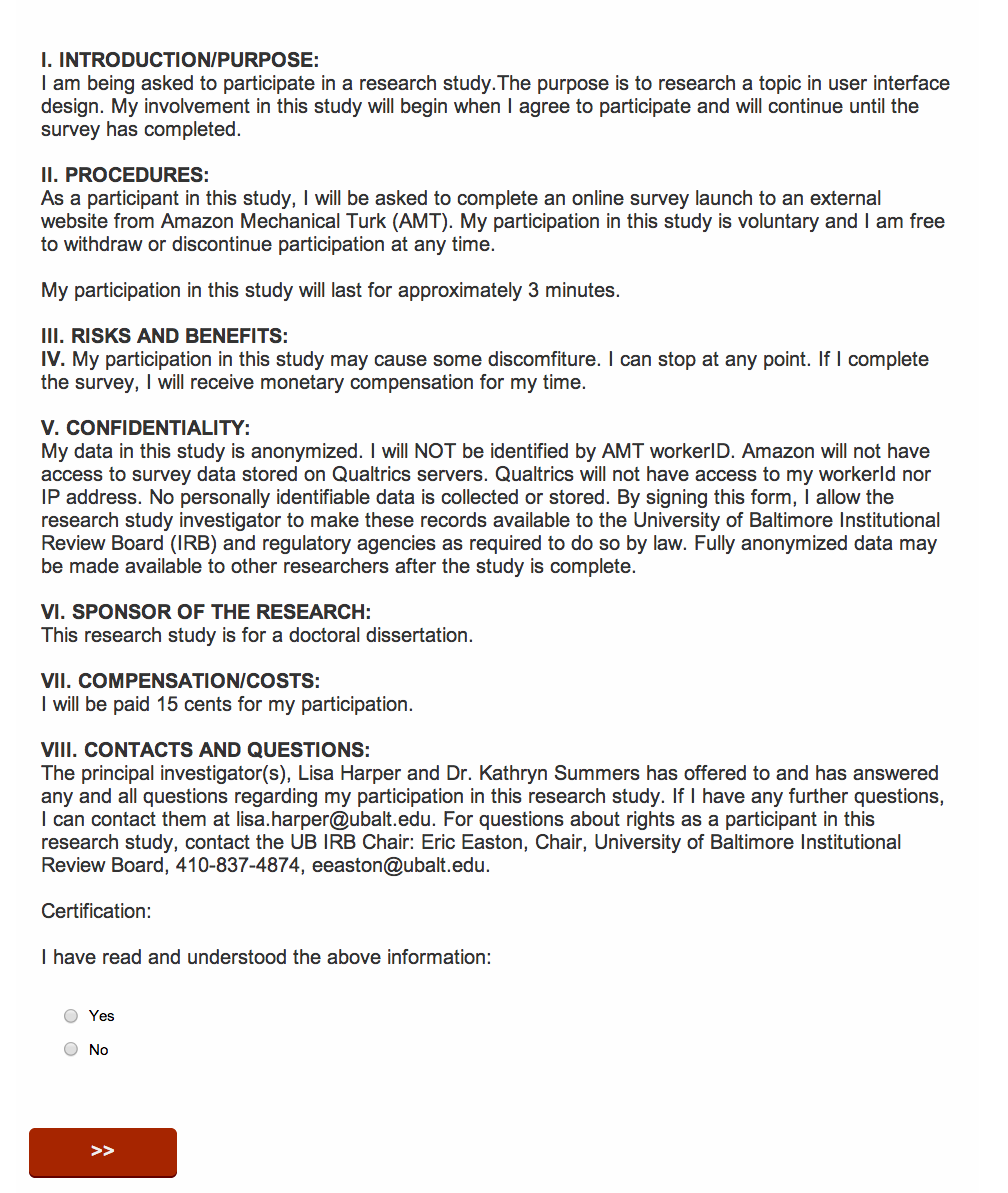
\includegraphics[scale=.40]{chapter4.tex/consent}
}
\end{figure}
%\setcounter{figure}{0} 
%
\chapter{AMT Terms of Service}
\label{amazon}
\begin{figure}[h!]
\centerline{
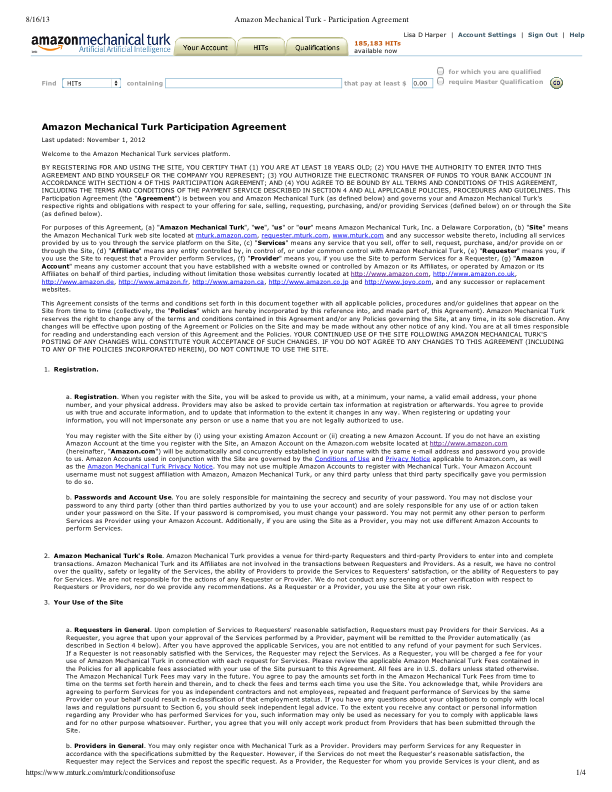
\includegraphics[scale=.6]{Appendices/amt-tos}
}
\end{figure}


%\setcounter{figure}{0} 
%
\chapter{Sample AMT Assignment Definition}
\label{assignment}
\lstset{numbers=none}
\begin{lstlisting}
title = Language study and demographic survey (3 min)
description: one task and then just a survey
keywords:survey, language

# how much you'll pay each subject
reward:.15

# how many subjects do you want
assignments:30

######################################
## HIT Timing Properties
######################################

# 60*10, 10 mins to finish a suvey
assignmentduration:600

# 60*60*24*2, 2 day to keep on mturk
hitlifetime:172800

# 10 seconds to auto approve the response
# 
autoapprovaldelay:10

######################################
## Qualification Properties
######################################

# user must have an approval rate of 90% or greater
qualification.1:000000000000000000L0
qualification.comparator.1:greaterthan
qualification.value.1:90
qualification.private.1:false

# user must be in the United States
qualification.2:00000000000000000071
qualification.comparator.2:equalto
qualification.locale.2:US
qualification.private.2:true
\end{lstlisting}


%\setcounter{figure}{0} 
%%**************************************************************
% Appendix
%*******************************************************
% If problems with the headers: get headings in appendix etc. right
%\markboth{\spacedlowsmallcaps{Appendix}}{\spacedlowsmallcaps{Appendix}}
\chapter{Survey Response}
\label{survey-response}
%%% LyX 2.0.6 created this file.  For more info, see http://www.lyx.org/.
%% Do not edit unless you really know what you are doing.
%\documentclass[english]{article}
%\usepackage[T1]{fontenc}
%\usepackage[latin9]{inputenc}
%\usepackage{longtable}
%\makeatletter

%%%%%%%%%%%%%%%%%%%%%%%%%%%%%% LyX specific LaTeX commands.
%% Because html converters don't know tabularnewline
%\providecommand{\tabularnewline}{\\}

%\makeatother

%\usepackage{babel}
%\begin{document}

%\setlength\LTleft{-30pt}            % default: \fill
%\setlength\LTright{-30pt}           % default: \fill
\footnotesize
\begin{longtable}{p{4cm} p{4cm}}
%\caption{Demographics (All Studies Combined)} \\
\textbf{Category} & \textbf{Percentage}\tabularnewline
\hline 
\hline 
\textbf{Age} & \tabularnewline
\hline 
18-24 & 28\%\tabularnewline
25-34 & 45\%\tabularnewline
35-49 & 20\%\tabularnewline
50-64 & 7\%\tabularnewline
64+ & 0\%\tabularnewline
\hline 
\textbf{Gender} & \tabularnewline
\hline 
Male & 53\%\tabularnewline
Female & 47\%\tabularnewline
\hline 
\textbf{Ethnic Identity} & \tabularnewline
\hline 
American Indian / Native American & 1\%\tabularnewline
Asian or Pacific Islander & 10\%\tabularnewline
Black / African American & 7\%\tabularnewline
Hispanic or Latin American & 7\%\tabularnewline
White / Caucasian & 73\%\tabularnewline
Near Eastern or Arabic & 0\%\tabularnewline
Other & 2\%\tabularnewline
\hline 
\textbf{Native Language} & \tabularnewline
\hline 
English & 97\%\tabularnewline
Other & 3\%\tabularnewline
\hline 
\textbf{English} & \tabularnewline
\hline 
A little English & 0\%\tabularnewline
Some English & 0\%\tabularnewline
Fluent English & 60\%\tabularnewline
Near-native English & 40\%\tabularnewline
\hline 
\textbf{Education} & \tabularnewline
\hline 
Some High School & 1\%\tabularnewline
High School Graduate & 13\%\tabularnewline
Some College / Associate Degree & 40\%\tabularnewline
College Degree & 37\%\tabularnewline
Post-graduate Degree & 9\%\tabularnewline
\hline 
\textbf{Income} & \tabularnewline
\hline 
Under 20,000 & 34\%\tabularnewline
20,000 - 30,000 & 19\%\tabularnewline
30,000 - 40,000 & 15\%\tabularnewline
40,000 - 50,000 & 10\%\tabularnewline
50,000+ & 22\%\tabularnewline
\hline 
\textbf{IT Job} & \tabularnewline
\hline
Yes & 20\%\tabularnewline
No & 80\%\tabularnewline
\hline 
\textbf{Internet Usage} & \tabularnewline
\hline 
Fewer than 4 hours per week & 2\%\tabularnewline
4-10 hours per week & 11\%\tabularnewline
10-25 hours per week & 30\%\tabularnewline
25+ hours per week & 57\%\tabularnewline
\hline 
\textbf{Shop Online} & \tabularnewline
\hline 
Never & 1\%\tabularnewline
Rarely & 17\%\tabularnewline
Sometimes & 30\%\tabularnewline
Often & 52\%\tabularnewline
\hline 
\textbf{Sense of Privacy in Public} & \tabularnewline
\hline 
Not private & 29\%\tabularnewline
A Little private & 30\%\tabularnewline
Somewhat private & 29\%\tabularnewline
Private & 9\%\tabularnewline
Very private & 3\%\tabularnewline
\hline 
\textbf{Sense of Privacy at Home} & \tabularnewline
\hline 
Not private & 4\%\tabularnewline
A Little private & 10\%\tabularnewline
Somewhat private & 23\%\tabularnewline
Private & 37\%\tabularnewline
Very private & 26\%\tabularnewline
\hline 
\textbf{Importance of Online Privacy } & \tabularnewline
\hline 
Not much of an issue & 7\%\tabularnewline
Somewhat important & 51\%\tabularnewline
Really important & 42\%\tabularnewline
\hline 
\textbf{Steps to Protect Privacy} & \tabularnewline
\hline 
Don't know how to protect & 8\%\tabularnewline
Know how but not consistent & 49\%\tabularnewline
Know how and take measures & 43\%\tabularnewline
\hline 
\textbf{Know what a tracking cookie is} & \tabularnewline
\hline 
Yes & 91\%\tabularnewline
No & 9\%\tabularnewline
\hline 
\textbf{DNT means...} & \tabularnewline
\hline 
Do not show targeted advertising & 20\%\tabularnewline
Do not track across sites & 54\%\tabularnewline
Do not track on this site & 47\%\tabularnewline
Do not collect information & 48\%\tabularnewline
Do not store information & 43\%\tabularnewline
\hline 
\textbf{Would Turn off Tracking if Easy?} & \tabularnewline
\hline 
Yes & 91\%\tabularnewline
No & 9\%\tabularnewline
\hline 
\textbf{Browser Configured Opt-Out} & \tabularnewline
\hline 
Yes & 55\%\tabularnewline
No & 45\%\tabularnewline
\hline 
\textbf{Use a Browser Plugin for Privacy Protection} & \tabularnewline
\hline 
Yes & 73\%\tabularnewline
No & 27\%\tabularnewline
\hline 
\textbf{Total} & \textbf{1158}\tabularnewline
\hline 
\end{longtable}
%\end{document}

%% LyX 2.0.6 created this file.  For more info, see http://www.lyx.org/.
%% Do not edit unless you really know what you are doing.
%\documentclass[english]{article}
%\usepackage[T1]{fontenc}
%\usepackage[latin9]{inputenc}

%\makeatletter

%%%%%%%%%%%%%%%%%%%%%%%%%%%%%% LyX specific LaTeX commands.
%% Because html converters don't know tabularnewline
%\providecommand{\tabularnewline}{\\}

%\makeatother

%\usepackage{babel}
%\begin{document}

\begin{longtable}{p{4cm} p{4cm} p{3cm}}
\caption{Aggregate Demographic Profile and Survey Response} \\
\textbf{Category} & \textbf{Experiment 3} & \textbf{Total}\tabularnewline
\hline 
\hline 
\textbf{Age} &  & \tabularnewline
\hline 
18-24 & 29\% & 28\%\tabularnewline
25-34 & 44\% & 45\%\tabularnewline
35-49 & 17\% & 20\%\tabularnewline
50-64 & 10\% & 7\%\tabularnewline
64+ & 0\% & 0\%\tabularnewline
\hline 
\textbf{Gender} &  & \tabularnewline
\hline 
Male & 63\% & 53\%\tabularnewline
Female & 37\% & 47\%\tabularnewline
\hline 
\textbf{Ethnic Identity} &  & \tabularnewline
\hline 
American Indian / Native American & 0\% & 1\%\tabularnewline
Asian or Pacific Islander & 10\% & 10\%\tabularnewline
Black / African American & 3\% & 7\%\tabularnewline
Hispanic or Latin American & 5\% & 7\%\tabularnewline
White / Caucasian & 82\% & 73\%\tabularnewline
Near Eastern or Arabic & 0\% & 0\%\tabularnewline
Other & 2\% & 2\%\tabularnewline
\hline 
\textbf{Native Language} &  & \tabularnewline
\hline 
English & 99\% & 97\%\tabularnewline
Other & 1\% & 3\%\tabularnewline
\hline 
\textbf{English} &  & \tabularnewline
\hline 
A little English & 0\% & 0\%\tabularnewline
Some English & 0\% & 0\%\tabularnewline
Fluent English & 0\% & 60\%\tabularnewline
Near-native English & 100\% & 40\%\tabularnewline
\hline 
\textbf{Education} &  & \tabularnewline
\hline 
Some High School & 1\% & 1\%\tabularnewline
High School Graduate & 17\% & 13\%\tabularnewline
Some College or Associate Degree & 39\% & 40\%\tabularnewline
College Degree & 35\% & 37\%\tabularnewline
Post-graduate Degree & 8\% & 9\%\tabularnewline
\hline 
\textbf{Income} &  & \tabularnewline
\hline 
Under 20,000 & 30\% & 34\%\tabularnewline
20,000 - 30,000 & 25\% & 19\%\tabularnewline
30,000 - 40,000 & 13\% & 15\%\tabularnewline
40,000 - 50,000 & 13\% & 10\%\tabularnewline
50,000+ & 20\% & 22\%\tabularnewline
\hline 
\textbf{IT Job} &  & \tabularnewline
\hline
Yes & 21\% & 20\%\tabularnewline
No & 79\% & 80\%\tabularnewline
\hline 
\textbf{Internet Usage} &  & \tabularnewline
\hline 
Fewer than 4 hours per week & 1\% & 2\%\tabularnewline
4-10 hours per week & 13\% & 11\%\tabularnewline
10-25 hours per week & 41\% & 30\%\tabularnewline
25+ hours per week & 45\% & 57\%\tabularnewline
\hline 
\textbf{Shop Online} &  & \tabularnewline
\hline 
Never & 1\% & 1\%\tabularnewline
Rarely & 20\% & 17\%\tabularnewline
Sometimes & 59\% & 30\%\tabularnewline
Often & 21\% & 52\%\tabularnewline
\hline 
\textbf{Sense of Privacy in Public} &  & \tabularnewline
\hline 
Not private & 31\% & 29\%\tabularnewline
A Little private & 34\% & 30\%\tabularnewline
Somewhat private & 23\% & 29\%\tabularnewline
Private & 11\% & 9\%\tabularnewline
Very prvate & 1\% & 3\%\tabularnewline
\hline 
\textbf{Sense of Privacy at Home} &  & \tabularnewline
\hline 
Not private & 5\% & 4\%\tabularnewline
A Little private & 15\% & 10\%\tabularnewline
Somewhat private & 23\% & 23\%\tabularnewline
Private & 34\% & 37\%\tabularnewline
Very prvate & 24\% & 26\%\tabularnewline
\hline 
\textbf{Importance of Online Privacy } &  & \tabularnewline
\hline 
Not much of an issue & 8\% & 7\%\tabularnewline
Somewhat important & 50\% & 51\%\tabularnewline
Really important & 42\% & 42\%\tabularnewline
\hline 
\textbf{Steps to Protect Privacy} &  & \tabularnewline
\hline 
Don't know how to protect & 12\% & 8\%\tabularnewline
Know how but not consistent & 38\% & 49\%\tabularnewline
Know how and take measures & 50\% & 43\%\tabularnewline
\hline 
\textbf{Know what a tracking cookie is} &  & \tabularnewline
\hline 
Yes & 90\% & 91\%\tabularnewline
No & 10\% & 9\%\tabularnewline
\hline 
\textbf{DNT means...} &  & \tabularnewline
\hline 
Do not show targeted advertising & 17\% & 20\%\tabularnewline
Do not trakc across sites & 44\% & 54\%\tabularnewline
Do not track on this site & 49\% & 47\%\tabularnewline
Do not collect information & 39\% & 48\%\tabularnewline
Do not store information & 38\% & 43\%\tabularnewline
\hline 
\textbf{Would Turn off Tracking if Easy?} &  & \tabularnewline
\hline 
Yes & 88\% & 91\%\tabularnewline
No & 12\% & 9\%\tabularnewline
\hline 
\textbf{Browser Configured Opt-Out} &  & \tabularnewline
\hline 
Yes & 54\% & 55\%\tabularnewline
No & 46\% & 45\%\tabularnewline
\hline 
\textbf{Use a Browser Plugin for Privacy Protection} &  & \tabularnewline
\hline 
Yes & 70\% & 73\%\tabularnewline
No & 30\% & 27\%\tabularnewline
\hline 
\textbf{Total} & \textbf{100} & \textbf{1158}\tabularnewline
\end{longtable}
%\end{document}

%\setcounter{figure}{0} 
%
\chapter{Experiment 1 Conditions}
\label{exp1-conditions}
\begin{figure}[h!]
\centerline{
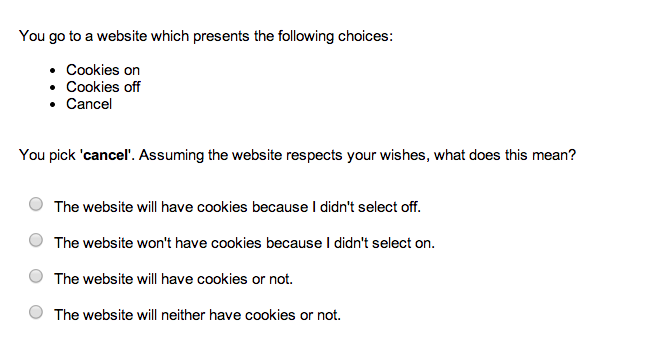
\includegraphics[scale=.5]{chapter5.tex/textnocpcookie}
}
\caption{Text, No Deontic Force, Cookie Condition}
\end{figure}


\begin{figure}[h!]
\centerline{
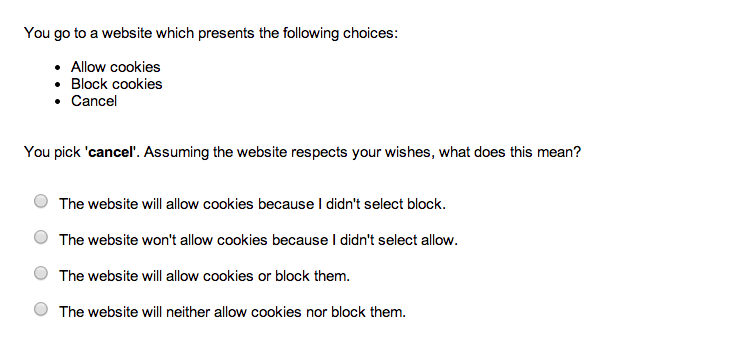
\includegraphics[scale=.5]{chapter5.tex/textcpcookie}
}
\caption{Text, Deontic Force, Cookie Condition}
\end{figure}


\begin{figure}[h!]
\centerline{
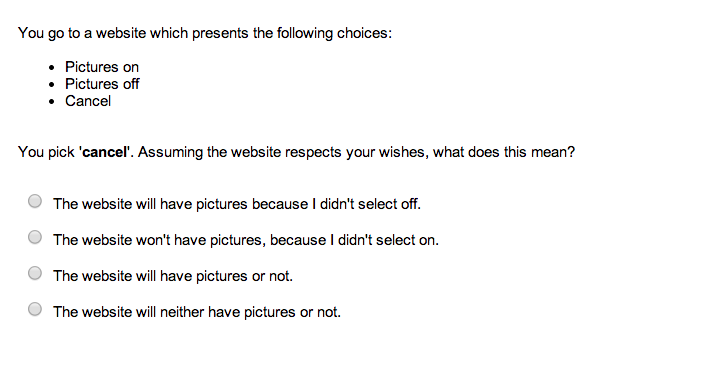
\includegraphics[scale=.5]{chapter5.tex/textnocppic}
}
\caption{Text, No Deontic Force, Picture Condition}
\end{figure}


\begin{figure}[h!]
\centerline{
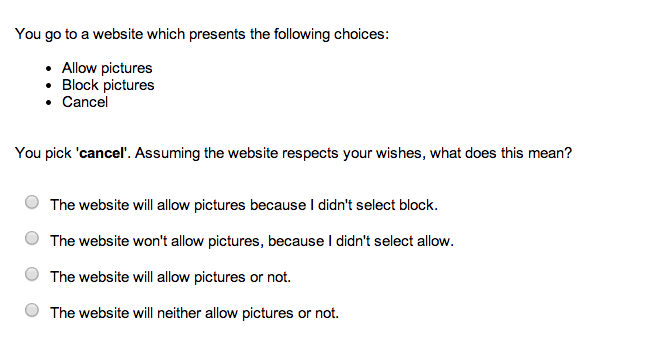
\includegraphics[scale=.5]{chapter5.tex/textcppic}
}
\caption{Text, Deontic Force, Picture Condition}
\end{figure}


\begin{figure}[h!]
\centerline{
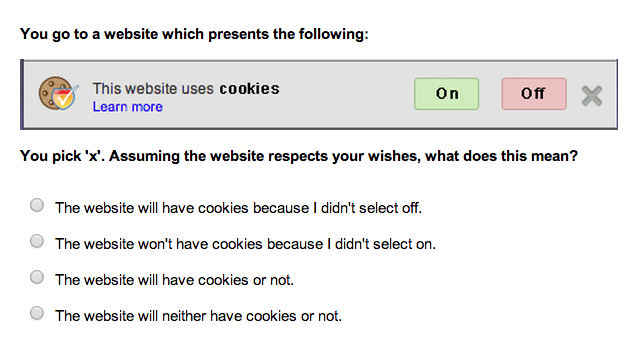
\includegraphics[scale=.5]{chapter5.tex/dialognocpcookie}
}
\caption{Mixed-Modal, No Deontic Force, Cookie Condition}
\end{figure}


\begin{figure}[h!]
\centerline{
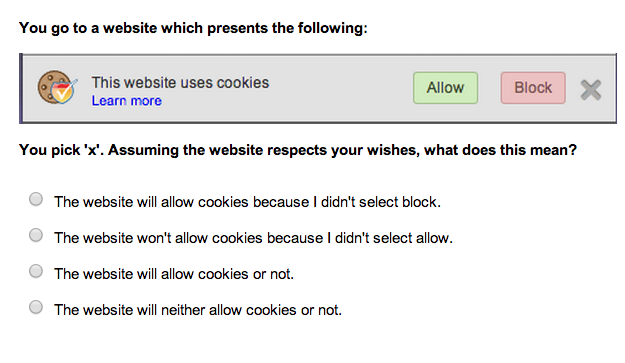
\includegraphics[scale=.5]{chapter5.tex/dialogcpcookie}
}
\caption{Mixed-Modal, Deontic Force, Cookie Condition}
\end{figure}



\begin{figure}[h!]
\centerline{
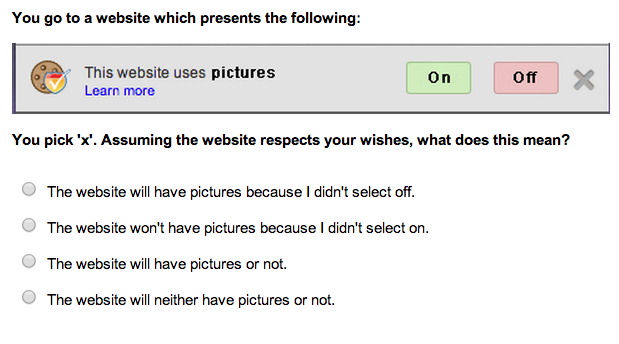
\includegraphics[scale=.5]{chapter5.tex/dialognocppic}
}
\caption{Mixed-Modal, No Deontic Force, Picture Condition}
\end{figure}


\begin{figure}[h!]
\centerline{
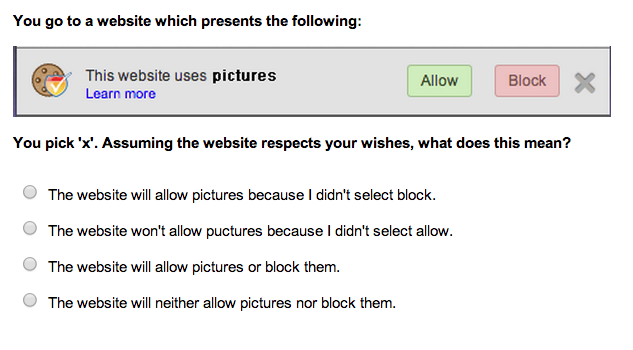
\includegraphics[scale=.5]{chapter5.tex/dialogcppic}
}
\caption{Mixed-Modal, Deontic Force, Picture Condition}
\end{figure}
%\setcounter{figure}{0} 
%
\chapter{Experiment 1 Raw Results}
\label{exp1-raw}
\begin{figure}[h!]
\centerline{
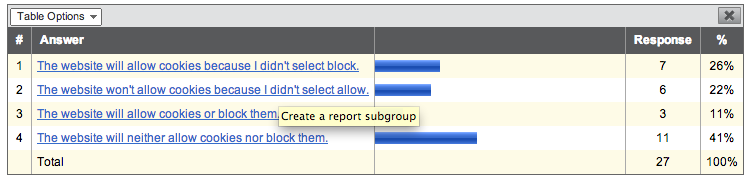
\includegraphics[scale=.44]{chapter5.tex/raw1}
}
\caption{Text, Deontic Force, Cookie Condition}
\end{figure}


\begin{figure}[h!]
\centerline{
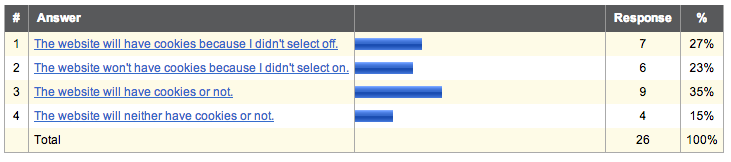
\includegraphics[scale=.45]{chapter5.tex/raw2}
}
\caption{Text, No Deontic Force, Cookie Condition}
\end{figure}


\begin{figure}[h!]
\centerline{
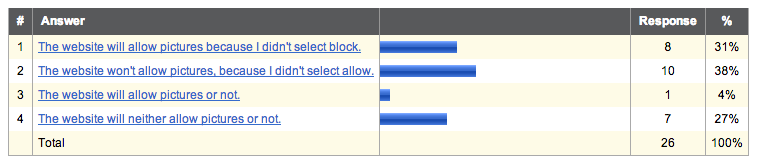
\includegraphics[scale=.45]{chapter5.tex/raw3}
}
\caption{Text, Deontic Force, Picture Condition}
\end{figure}


\begin{figure}[h!]
\centerline{
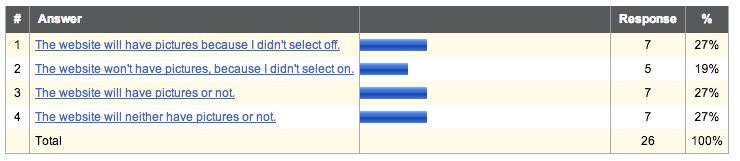
\includegraphics[scale=.45]{chapter5.tex/raw4}
}
\caption{Text, No Deontic Force, Picture Condition}
\end{figure}


\begin{figure}[h!]
\centerline{
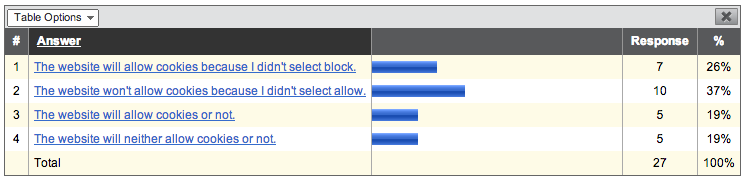
\includegraphics[scale=.44]{chapter5.tex/raw5}
}
\caption{Graphic, Deontic Force, Cookie Condition}
\end{figure}


\begin{figure}[h!]
\centerline{
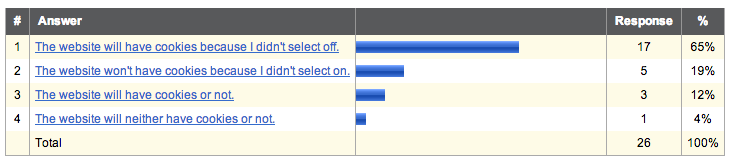
\includegraphics[scale=.45]{chapter5.tex/raw6}
}
\caption{Graphic, No Deontic Force, Cookie Condition}
\end{figure}


\begin{figure}[h!]
\centerline{
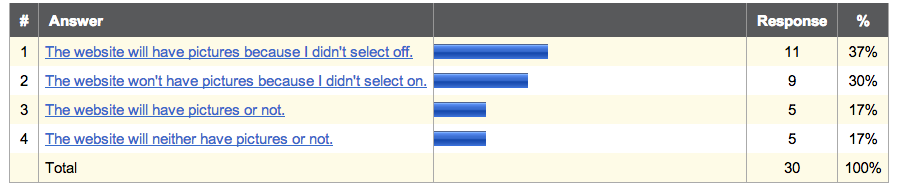
\includegraphics[scale=.38]{chapter5.tex/raw7}
}
\caption{Graphic, No Deontic Force, Picture Condition}
\end{figure}


\begin{figure}[h!]
\centerline{
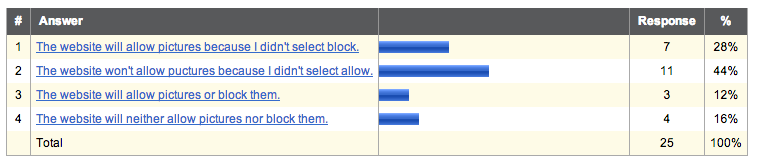
\includegraphics[scale=.45]{chapter5.tex/raw8}
}
\caption{Graphic, Deontic Force, Picture Condition}
\end{figure}
%\setcounter{figure}{0} 
%
\chapter{Participant Survey}
\label{survey}
%\begin{parbox}{\textwidth}
%\centering
%\begin{figure}
%\begin{sideways}
%\centerline{
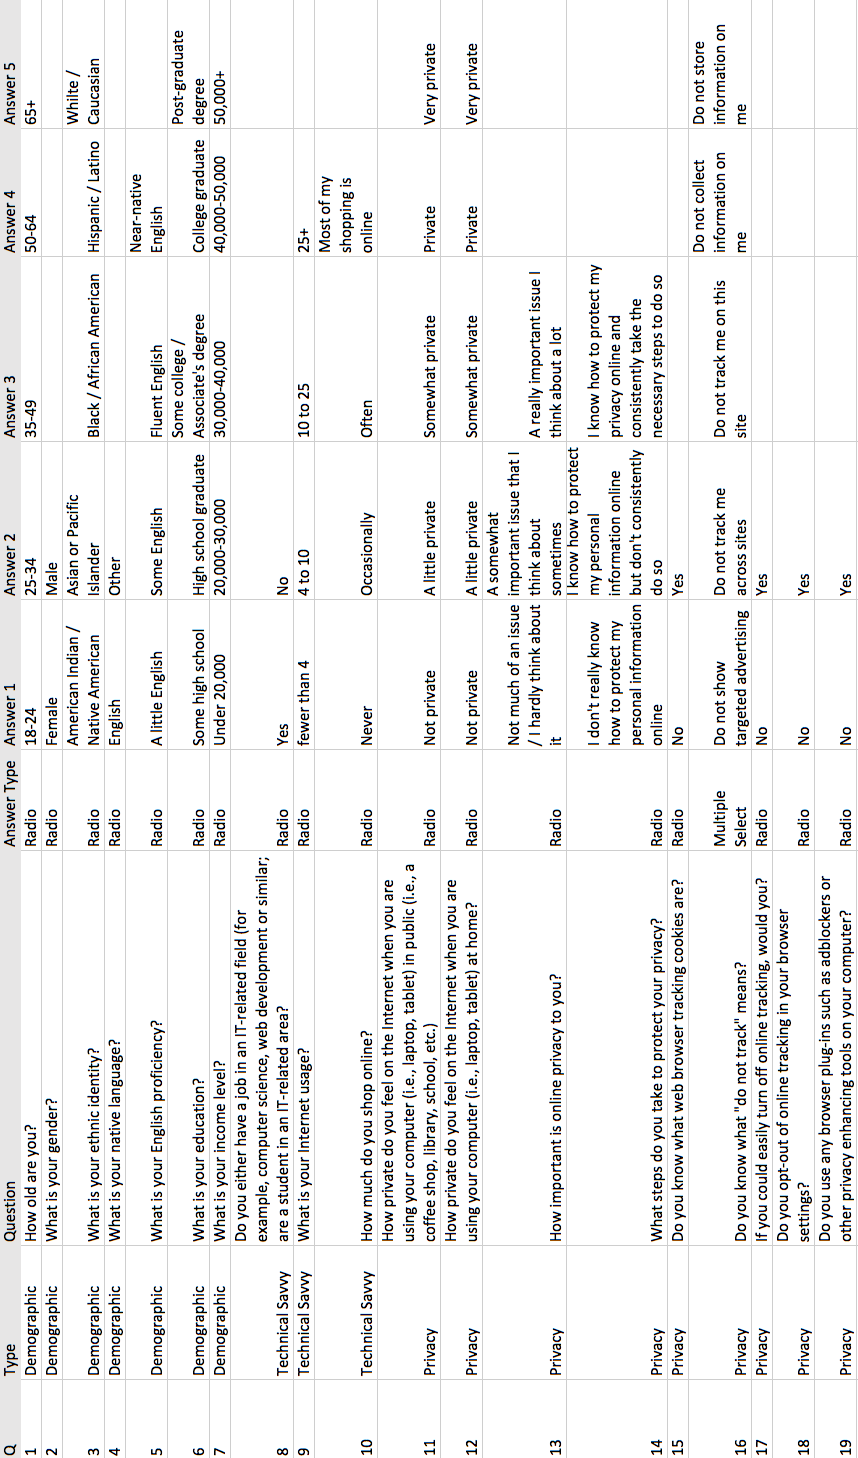
\includegraphics[scale=.38]{Appendices/survey-rotated}
%}
%\end{sideways}
%\end{figure}
%\end{parbox}

 %

%----------------------------------------------------------------------------------------
%	POST-CONTENT THESIS PAGES
%----------------------------------------------------------------------------------------

\cleardoublepage% Bibliography

\label{app:bibliography} % Reference the bibliography elsewhere with \autoref{app:bibliography}

\manualmark
\markboth{\spacedlowsmallcaps{\bibname}}{\spacedlowsmallcaps{\bibname}} 
\refstepcounter{dummy}

\addtocontents{toc}{\protect\vspace{\beforebibskip}} % Place the bibliography slightly below the rest of the document content in the table of contents
\addcontentsline{toc}{chapter}{\tocEntry{\bibname}}

%\bibliographystyle{plainnat}
%\bibliographystyle{apalike2}
\bibliographystyle{apacite}

%\bibliography{Bibliography}
\bibliography{bib} % Bibliography

\end{document}